

\documentclass[10pt]{sensys-proc}
\usepackage{graphicx}
\usepackage{balance}
\usepackage{comment}
\newcommand{\redcolor}[1]{\textcolor{red}{#1}}

\newcommand{\figref}[1]{Figure~\ref{#1}}
\newcommand{\secref}[1]{Section~\ref{#1}}
\newcommand{\tabref}[1]{Table~\ref{#1}}
\newcommand{\algoref}[1]{Algorithm~\ref{#1}}
\usepackage{graphicx}
\usepackage{subfig}
\usepackage{blindtext}
\usepackage{array}
\usepackage{caption}
\usepackage{url}
\usepackage{epstopdf}
\usepackage{multirow}
\usepackage{xcolor,colortbl}

\newcommand{\paradigm}{Sense-Local Store-Upload}

\newcommand{\paradigms}{Sense-Local Store-Upload~}

\newcommand{\pushline}{\Indp}
\definecolor{Gray}{gray}{0.91}
\newcolumntype{a}{>{\columncolor{Gray}}c}

\numberofauthors{2}

\author{
%
% The command \alignauthor (no curly braces needed) should
% precede each author name, affiliation/snail-mail address and
% e-mail address. Additionally, tag each line of
% affiliation/address with \affaddr, and tag the
%% e-mail address with \email.
\alignauthor Alice Security \\
        \affaddr{Department of Computer Science}\\
        \affaddr{University of Southern California}\\
       \email{alice@example.edu}
\alignauthor Bob Privacy \\
    \affaddr{Networked Embedded Systems Group}\\
    \affaddr{Swedish Institute of Computer Science}\\
    \email{bob@example.se}
}

\title{Its Different: Hitchiker’s Tryst with Energy Consumption Patterns in India}

\crdata{978-1-4503-1169-4}
\conferenceinfo{SenSys'13,} {November 11--15, 2013, Rome, Italy.}
\CopyrightYear{2013}

\begin{document}

\maketitle

\begin{abstract}
This paper provides a sample of a \LaTeX\ document for ACM Sensys. 
It complements the document \textit{Author's (Alternate) Guide to
Preparing ACM SIG Proceedings Using \LaTeX$2_\epsilon$\ and Bib\TeX}.
This source file has been written with the intention of being
compiled under \LaTeX$2_\epsilon$\ and BibTeX.

To make best use of this sample document, run it through \texttt{pdflatex}
and \texttt{bibtex} to directly produce a pdf document.
\end{abstract}

% A category with the (minimum) three required fields
\category{H.4}{Information Systems Applications}{Miscellaneous}
%A category including the fourth, optional field follows...
\category{D.2.8}{Software Engineering}{Metrics}[complexity measures, performance measures]

\terms{Delphi theory}

\keywords{ACM proceedings, \LaTeX, text tagging}

\section{Introduction+Related Work}
  \label{sec:intro}

\begin{itemize}
\item Why buildings must be targeted for energy \cite{evans09}
\item Importance of feedback \cite{darby}
\item Why we need deployments
\item Deployments- Residential, Office \cite{yuvraj_ipsn, batra}
\item Previous such residential deployments, some of which were presented in Buildsys itself \cite{hitchhiker_residential,hitchhiker_wsn,scale_wsn}
\item Some applications-NILM\cite{hart,survey1}, Fixture Finder \cite{fixturefinder}
\item Specific learnings from our deployment, some of them complement the ones given earlier \cite{hitchhiker_residential}
\begin{itemize}
\item Glowing LED in night 
\item Deployments should be transparent
\item Noisy server owing to dust (specific to developing countries)
\item Electricity failure- as a consequence all systems should be capable to restart upon resumption of electricity
\item Unreliable internet -Forcing to use Sense-Store-Upload paradigm
\item Normalization -Voltage fluctuation, different measurement by different instruments


\end{itemize}
\end{itemize}
Also deployment was maintained as an open source project. Shows how we faced issues and tackled them. Also contains metadata log provided by the end user.

\section{Deployment Overview}
Over the past year, we have deployed sensors across 22 homes. While 20 of these homes have been instrumented only with smart electricity meters, 2 homes have been extensively instrumented with upto 33 sensors measuring electricity, water and ambient parameters. \figref{fig:overall} shows the deployment in a 3 storey home where 33 sensors, 5 single board computers and 3 routers were used. 
\begin{figure}     
    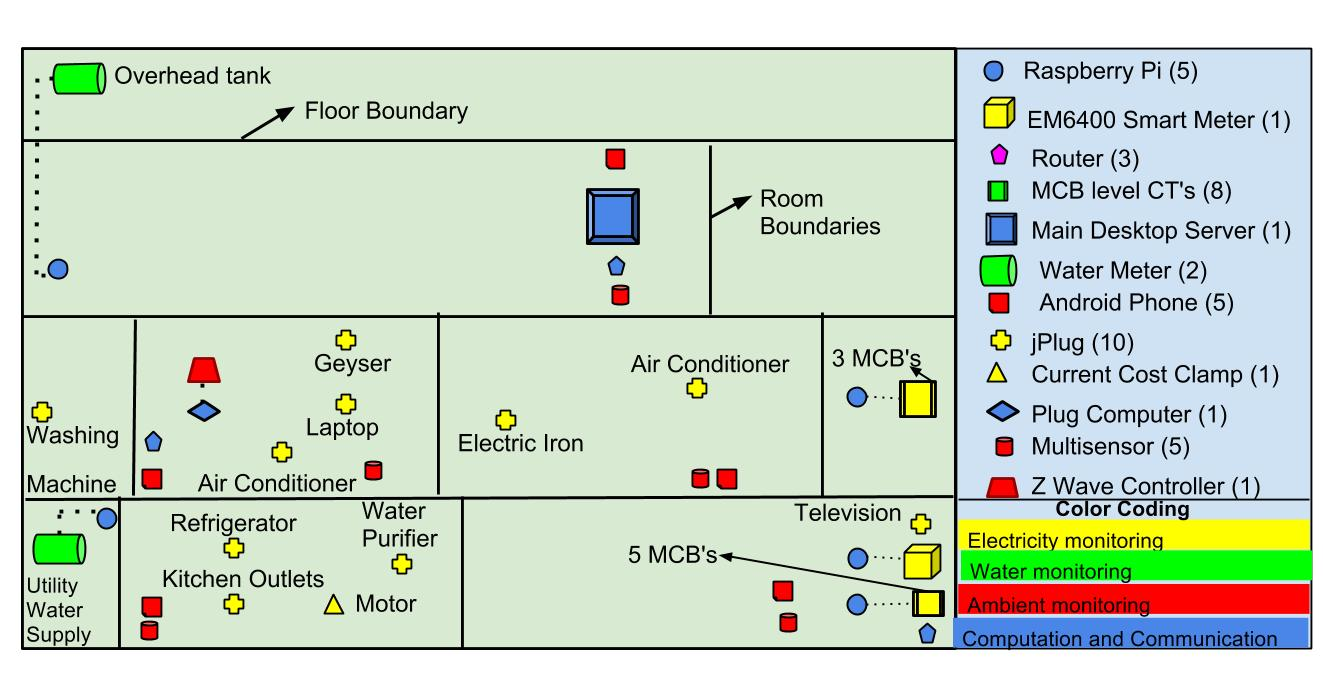
\includegraphics[scale=0.2]{./figures/overall_deployment.jpg}    
    \caption{Schematic showing overall home deployment}   
    \label{fig:overall}
   
\end{figure}
\subsection{Sensing Infrastructure}
\label{sec:sensing}
For our sensing, we took a ``leave no stone unturned'' approach, where  we chose to monitor as many physical parameters (such as ambient conditions, electricity usage, water usage) and non-physical parameters (such as network strength etc.). However, it must be noted, that we chose to deploy sensors in a way that home users can continue their regular routine without getting affected. We describe the various sensors used in our deployments below:

\noindent\textbf{Electricity monitoring:} A typical home electricity setup involves a meter which is installed by utility companies and measures overall electricity usage. Further electric cabling is divided into various Miniature Circuit Breakers (MCB's) which control separate circuits. Typical installations involve putting separate MCB's for heavier loads such as air conditioners and clubbing various lights, fans and other smaller loads into separate MCB. Further each individual appliance is controlled via a switch. There are two types of appliances- i) plug loads like refrigerator and electric iron, which need to be physically ``plugged" into the sockets; ii) loads like lights and fans, which do not need to be ``plugged" in by the user. We highlight the above described home electricity distribution in \figref{fig:overall}. We have 3 different resolutions at which electricity can be monitored:
\begin{enumerate}
\item \textbf{Meter level:} We use Schneider Electric EM6400\footnote{\url{www.goo.gl/01edPS}} smart meter to instrument the main power supply. While cheaper variants from the same company were available, we chose to use EM6400 as it also provides reactive power. This additional information has been known to be useful for NILM applications\cite{hart}. \figref{fig:em6400} shows EM6400 smart meter deployed in the electricity panel. We had to put 30:1 ratio CT on the power mains coming from the grid to ensure that the load current was transformed to be within EM6400's permissible limits. EM6400 allows reading various registers to measure more than 40 parameters including: voltage, current, phase, power (apparent, real, reactive) and various other parameters, using Modbus over RS485 serial link.

\item \textbf{Circuit level:} We used our in-house developed Current transformer (CT) based monitoring circuits which can be clamped to individual MCB's. \redcolor{Manoj write 1-2 lines about this circuit}. CT deployment is shown in \figref{fig:ct}. These CT's provide information about a circuit's current usage. We exposed a serial interface to log this current data.

\item \textbf{Appliance level:} We used jPlug\footnote{A variant of nPlug\cite{nplug}} to measure individual appliance power consumption for 9 plug-load type appliances. We also used Current Cost based CT to measure the power consumption for electric motor (used to pump water), which is not a plug-load, yet has significant power consumption (approx. 700 Watts). jPlug and Current Cost CT deployment are shown in \figref{fig:jplug} and \figref{fig:cc} respectively. jPlug makes a HTTP POST connection to log data. Current Cost exposes apparent power data over the serial port.
\end{enumerate}
More details regarding sensors used for electricity monitoring are provided in \tabref{tab:sensing}.

\noindent \textbf{Water monitoring:} There are few differences in home water distribution in India when compared to developed countries. In India, there are separate water lines for drinkable and non-drinkable water. Also, overhead water tanks (typically 1000 liters capacity) are used to store water. Electric motors are used to push water against gravity to be stored in the tank. Thus, the flow can be summarized as follows: 1) Water from utility comes to the home; 2) Electric motor is used to aid in pumping the water up to the tank; 3) Water flows downward from the tank whenever water is consumed. Thus, we put a water meter at the inlet (coming from the utility) and the outlet from the water tank (flowing downwards) to capture the incoming (from utility) and outgoing (from tank) water consumption. 


Digital water meters are very expensive and are not easily available in India. Thus, we chose to use Zenner Aquamter's multijet\footnote{\url{www.aquametwatermeters.com/multijet.html}}, which are analog in-line water meters, which measure water volume flowing through them. These water meters have a 4 ma current loop \redcolor{Manoj: Add details} and send a pulse every few liters. The precision is based on the quality of the sensor and the diameter of the water pipe. The water meter we used for overhead tank gives a pulse every 10 liters, whereas the one used for inlet supply from utility gives a pulse every 1 liter. These pulses can be measured using the circuit diagram for 4 ma loop shown in ... \figref{fig:water_meter} shows the water meter deployed inline at the overhead tank.

\noindent \textbf{Ambient conditions monitoring:} We used HomeSeer HSM100\footnote{\url{www.homeseer.com/pdfs/guides/HSM100_Release_Notes.pdf}} based multisensors for monitoring motion, light and temperature. While motion is reported in event-driven fashion (i.e. whenever there is change in motion status, reading is reported), temperature and light are polled at 1 Hz. This multisensor uses the well known ZWave\footnote{\url{http://en.wikipedia.org/wiki/Z-Wave}} protocol for communication. We also place Android phones at fixed locations and ran FunF journal\footnote{\url{http://www.funf.org/journal.html}} to log ambient parameters such as light and  sound level.

\noindent \textbf{Miscellaneous:} Android phones, in addition to measuring ambient conditions, were also logging nearby bluetooth and wireless devices and strength of cell-tower signal. All home occupants were requested to keep their phone's bluetooth on during the duration of the experiment. We also logged outside weather conditions such as temperature, humidity and wind speed using publicly available API's from weather monitoring stations. We believe that this data can be used for many applications including: energy-apportionment (i.e. assigning energy usage to different occupants within the home) and localization.

\noindent Sensing infrastructure is summarized in \tabref{tab:sensing}.


\begin{table*}
\caption{Sensing Infrastructure}

\label{tab:sensing}
\tabcolsep=0.015cm
\begin{tabular}{|l|l|l|l|l|l|l|}
\hline
Sensor&Sensor&Sampling&Resolution&Qua-&Commu-&Observed\\
name&type&frequency&&ntity&nication&parameters\\
&&(Hz)&&&&\\
\hline

EM6400&Electric Meter&1&Home&1&RS 485 Serial&Voltage, Current, Frequency,\\ 
&&&&&&Phase, Power(Active, Reactive \\ 
&&&&&&and Apparent), Energy\\ \hline
Aquamet &Water Meter&5&Main supply&2&Direct wire con-&10 liter events for tank and \\ 
multijet&&& and tank&&nection to GPIO&1 liter events for main supply\\ \hline
Homeseer &Ambient multisensors&Light, temperature: 1&Room &6&ZWave&Light, temperature\\ 
     HSM-100           &&PIR: event based&&&& and motion\\ \hline
Android&Ambient multisensors&Audio, light: 0.05&Room&5&Manually&Audio features, light, nearby \\ 
phones&and network&Nearby WiFi, cellular,&&&transfer files&bluetooth, cell-tower, WiFi\\ 
&& bluetooth: 0.001&&&to PC&\\ \hline
Prototype CT&Electricity meter&20&MCB&8&Serial&Current \\\hline
jPlug&Electricity meter & 1 &Appliance&10&WiFi&Voltage, Current, Frequency,\\ 
&&&&&&Power (Active and Apparent),\\
&&&&&& Energy, Phase\\ \hline	
Current Cost&Electricity meter&0.1&Appliance&1&Serial&Apparent power\\ \hline


\end{tabular}


\end{table*}

\subsection{Communication and Computation Infrastructure}
In our experience we found that using a desktop computer for collecting data from sensors would be an overkill in terms of cost, processing power and physical space used. Although microcontrollers are cheap and occupy little space, they do not expose enough abstractions for high level programming and are often difficult to debug and are inherently hard to multi task. We thus decided to use Single Board Computers (SBC's) for sensor data collection. We used Raspberry Pi\footnote{\url{www.raspberrypi.org}} (RPi) and Ionics Stratus\footnote{\url{www.ionics-ems.com/plugtop/stratus.html}} as our SBC's. These SBC's are available for about the same cost (25 \$) as microcontrollers. Moreover, they possess 700 MHz ARM processors and allow one to use Linux based distributions. Thus, one can use the full Linux stack and code in higher level languages such as Python. These SBC's run from SD cards and one can choose the SD card size based on usage. 

We used a total of 6 SBC's of which 5 were RPi and 1 was Ionics Stratus plug computer. We used a 2 GHz Desktop PC running Linux as the main server where all the data was stored. The software stack running on the SBC's and how they interacted with the main server and collected data from different sensors is described below:

\noindent \textbf{EM6400 smart meter data collection:} EM6400 allows data to be read from its registers over RS485 using Modbus protocol. We connected a RPi to EM6400 using RS485-USB converter which exposes serial interface over USB on RPi. We developed a custom Python program based on pyModbus\footnote{\url{www.github.com/bashwork/pymodbus}} library which would serially read 80 registers, using Modbus protocol, to compute 40 electrical parameters as described in \tabref{tab:sensing}. It would store these 40 parameters along with UTC timestamp in a CSV file. A new CSV would be created every 15 minutes. A background program would periodically try to upload CSV files older than 15 minutes, to the main server, where the data would be dumped in MySQL database.

\noindent \textbf{Current Cost data collection:} Although Current Cost has its own cloud based API platforms, we chose to collect data from it locally, in order to avoid data losses occurring due to network failures. Current Cost provides power data in xml format over the serial interface. We thus connected the USB cable-out from the Current Cost receiver to RPi and wrote a simple Python script to read data serially using pySerial\footnote{\url{www.pyserial.sourceforge.net}} and store it in a CSV file alongwith UTC timestamp. CSV creation and uploading to central server was done in a similar fashion as was done for EM6400.

It must be noted that we used the same model- create new CSV periodically, upload older CSV periodically to main server where they are dumped into MySQL for all sensors. We call this model \paradigms and describe it in more details in section \secref{sec:architecture}

\noindent \textbf{MCB data collection:} Our custom built CT based sensor solution for collecting current data from different MCB's exposes data serially which is read using pySerial on a RPi and processed further using \paradigm.

\noindent \textbf{jPlug appliance data collection:} jPlug makes a HTTP post every second with upto 10 electrical parameters. We saved this data directly on the server machine where a web daemon listened to requests from jPlug and dumped them in MySQL.

\noindent \textbf{Water data collection:} Based on circuitry explained in \secref{sec:sensing}, we used GPIO header on RPi and wrote an interrupt driven program in Python to detect 10 liter and 1 liter events for the tank and supply water meters respectively. We found that noise introduced in the circuit due to long cable lengths led to a lot of false events. Thus, we modified our program and polled at a frequency of 5 Hz to obtain GPIO status and further processed this data using \paradigm.	

\noindent \textbf{Homeseer HSM100 data collection:} We wrote custom wrappers around OpenZWave\footnote{\url{www.code.google.com/p/open-zwave}} program to collect temperature and light information on a per second basis, and motion information based on events. ZWave controller which controls all the ZWave based sensors was connected to the plug computer over USB. Data was processed further using \paradigm. \figref{fig:plug} shows plug computer collecting ambient sensor data from ZWave controller.

\noindent \textbf{Android data collection:} We used FunF journal which would store data inside phone's SD card. We would take a dump once every 15 days and empty the SD card for further data collection.

\noindent \textbf{Weather data collection:} Electricity failure  and reliable Internet are well known problems in India and are highlighted in \secref{sec:learning}. Owing to these problems, we chose to collect weather data from 3 different weather stations, in our collaborator's institute in the USA.

In our deployment a lot of issues pertaining to SBC's were found. For instance, the OpenZWave program that we used would create log files for its own diagnostics. This eventually ate up the 512 MB flash drive space on the plug computer. We fixed this by deleting older logs. We also observed that the circuit for water meter was heating up RPi due to high current passing through the resistance. These led us to develop soft-sensor streams whereby we collected hard disk space, ping success, CPU utilized, RAM left, temperature of processor for all the computing devices including the server at regular intervals. These soft-sensor streams can be used for alerting mechanisms and can also be used for fault diagnoses. Similar soft-sensor streams have also been used in previous work\cite{hitchhiker_residential} where they used them for alerts.

We found that one WiFi router will not suffice for a 3 storey building. This has also been reported in previous work on residential deployments\cite{hitchhiker_residential}. We thus used 3 routers, where the router on the first floor acted as the host and routers on ground and second floor were bridged to it. More details regarding the need of multiple routers and network availability in homes is described in \secref{sec:learning}.




\subsection{System Architecture}	
\label{sec:architecture}
Various middleware systems such as sMAP\cite{smap}, Building Depot\cite{buildingdepot} and SensorAct\cite{Arjunan12} have been proposed in the past for sensor data collection. However, we found that they are not fine tuned to our needs arising from faulty internet, power failures, etc. Moreover, these systems provide a lot more features than we intend to use. Thus, based on our experience and previous work\cite{hitchhiker_residential}, where importance of simplifying the architecture are proposed, we propose \paradigm. \paradigms involves local storage and periodic data upload. As explained above, we used SBC's to collect data from sensors. This data was \textbf{locally stored} in form of comma separated value files (CSV) and was \textbf{periodically uploaded} to the main desktop server. In case the upload failed, it was retried the next time again. Each SBC had sufficient flash based local storage to accommodate sensor data for a few days. 

\begin{figure}     
    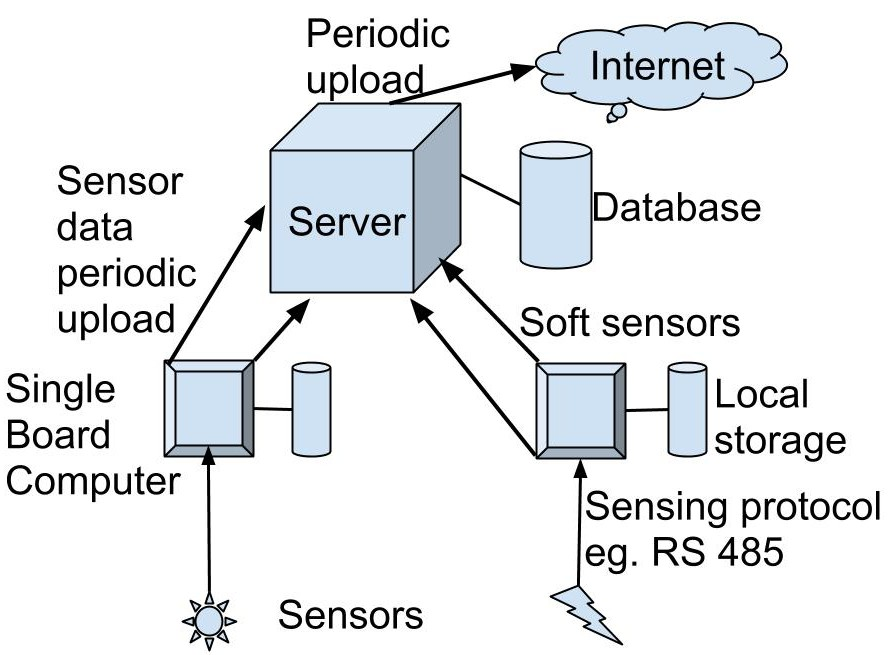
\includegraphics[scale=0.20]{./figures/architecture.jpg}    
    \caption{\paradigm}   
    \label{fig:architecture}   
\end{figure}

Web applications running on the server allowed a home user to locally visualize his data from multiple streams. Further, data from the server can be copied to cloud based servers such as Dropbox where applications such as analytics, alerts can be done, allowing outside users and specifically researchers to keep an eye on the deployment sitting in their labs. \figref{fig:architecture} explains \paradigms architecture. The salient features of our architecture are as follows:
\begin{itemize}
\item \textbf{Decoupled sensing and data uploading:} This ensures that an error in one does not prevent the other action from occuring correctly and thus allows easier debugging. Moreover, this design choice of decoupling comes from the well established principles of software engineering.
\item \textbf{Minimal internet requirement:} Internet is required \textbf{only} when outside researchers wish to view and analyze collected data in realtime. Internet failure does not have any impact on sensor data collection.
\item \textbf{Reduced load on server:} Since data is uploaded periodically in larger chunks rather than sending data for each sensor packet, computation and bandwidth requirements are greatly reduced.
\end{itemize}

\begin{figure*} 
    
    \subfloat[\scriptsize EM6400 Smart Meter]{
    \label{fig:em6400}
    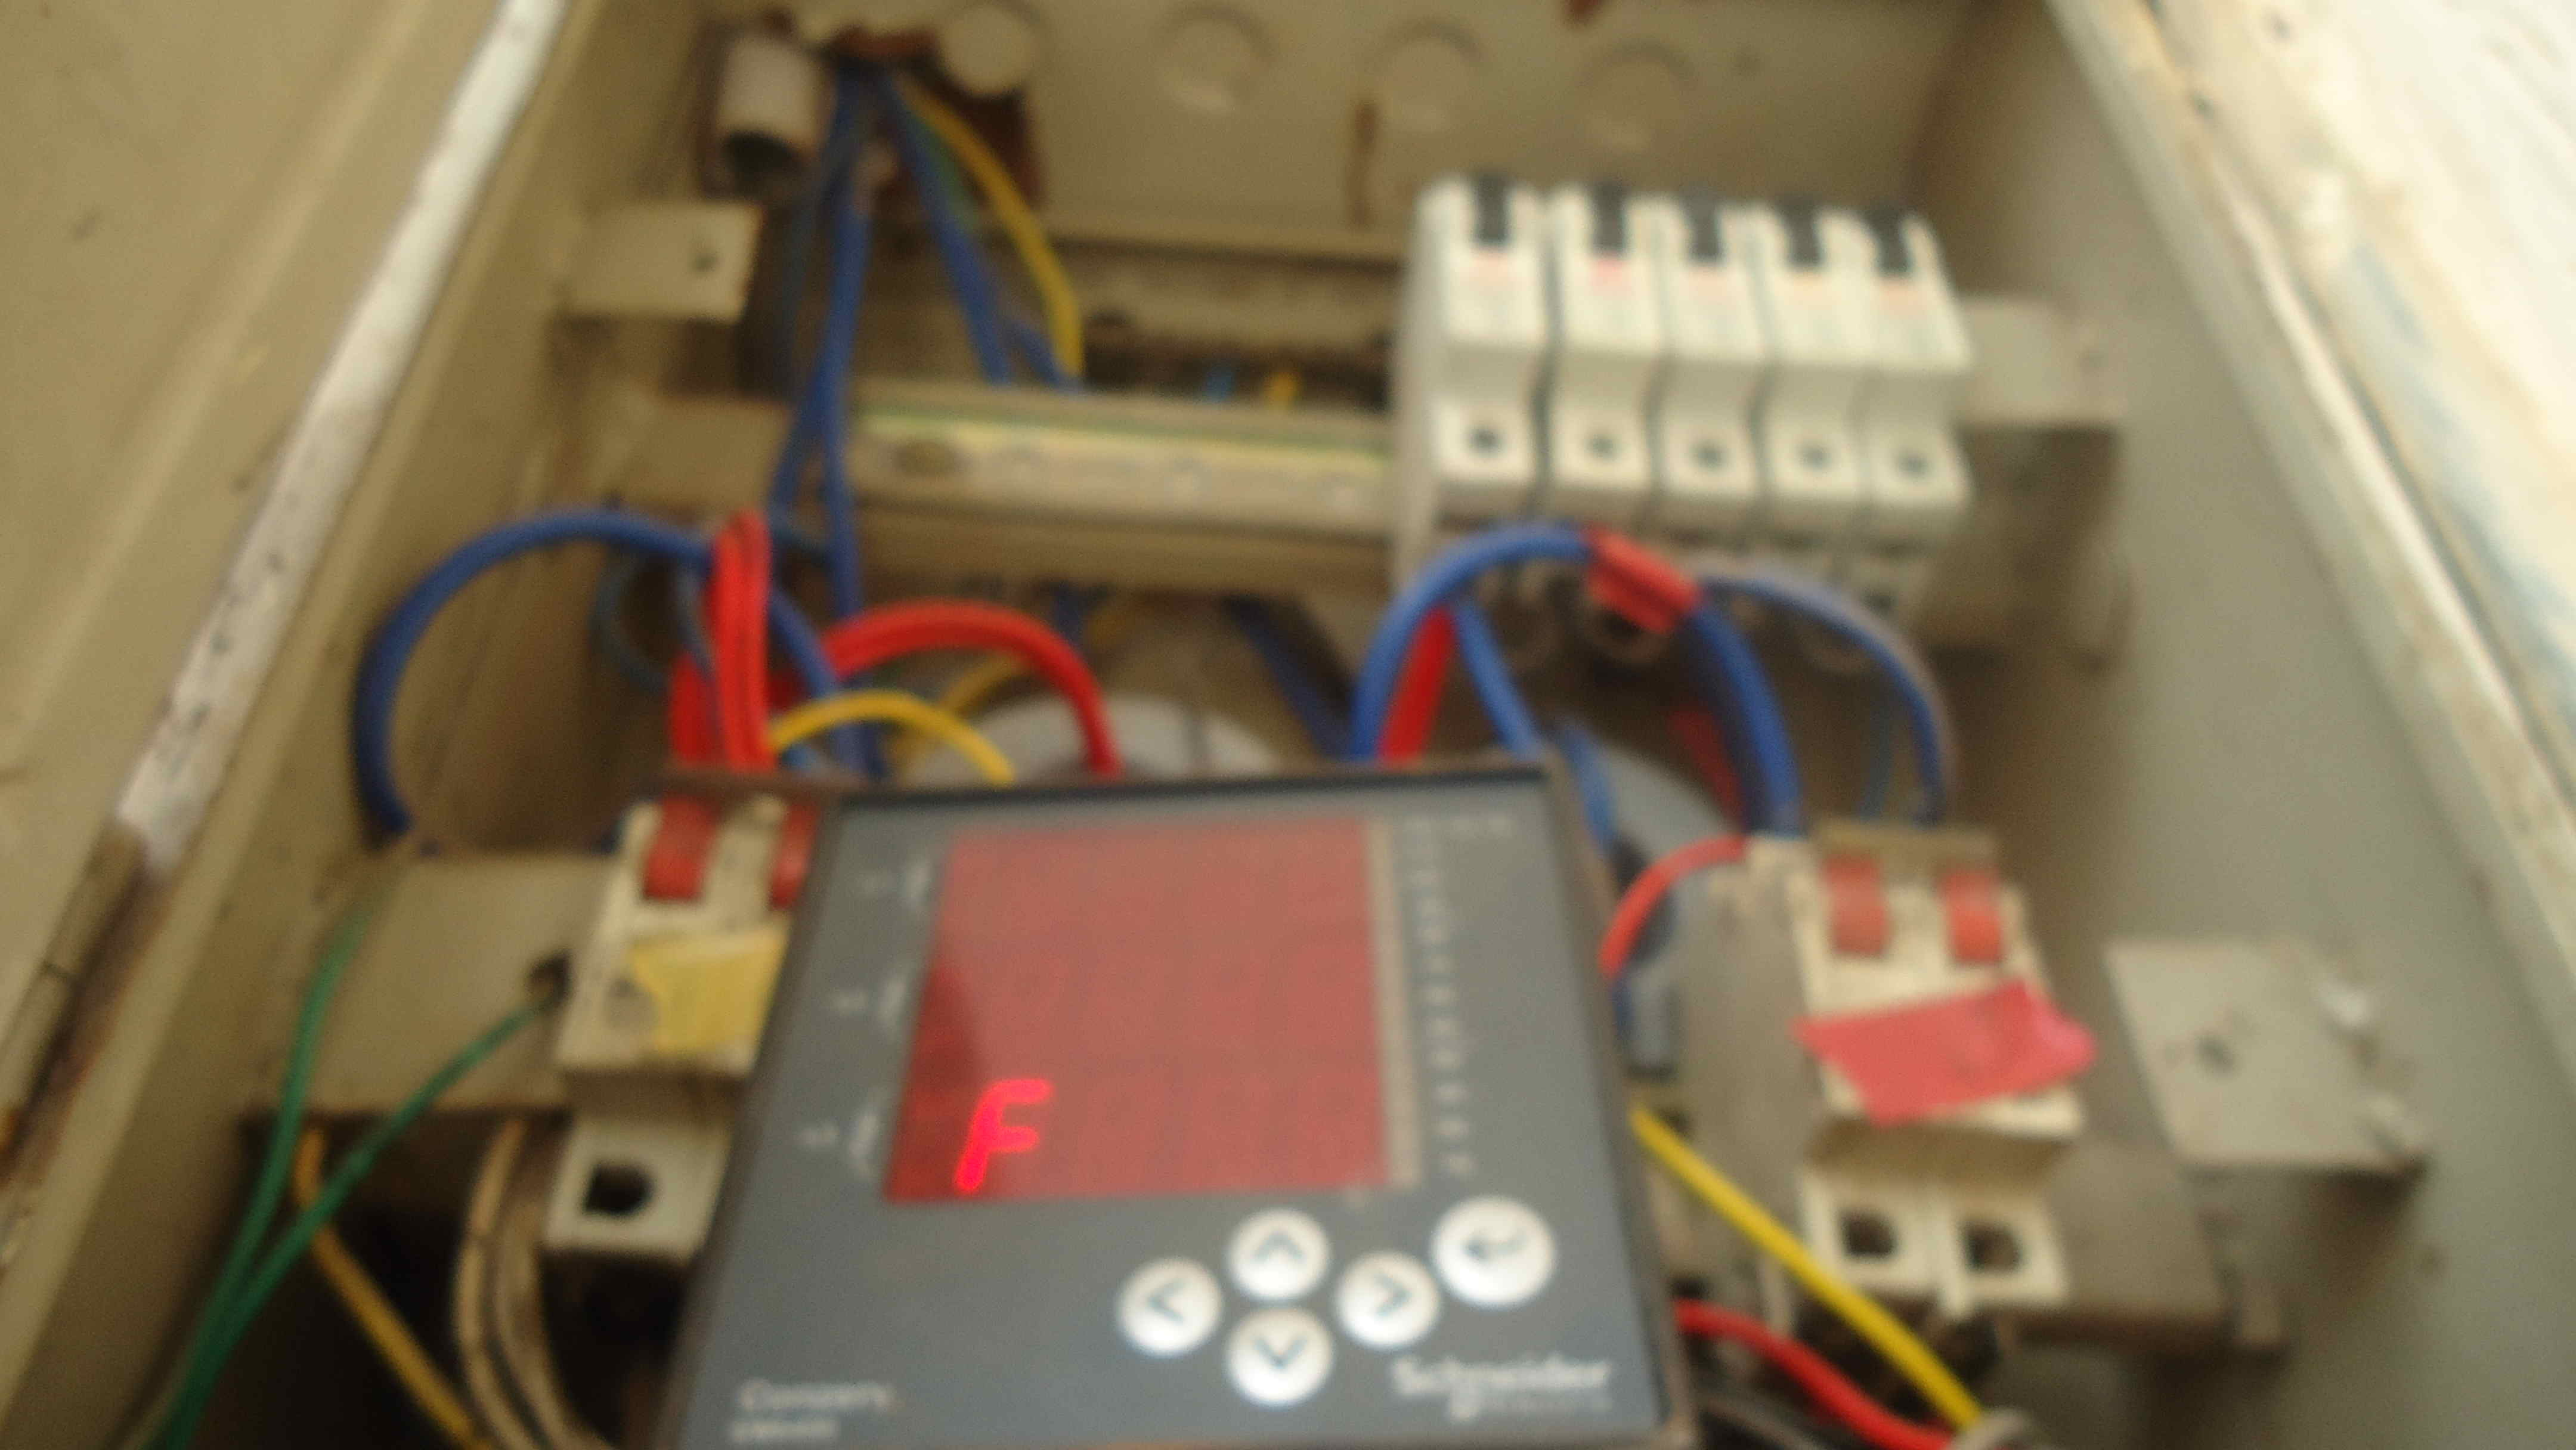
\includegraphics[scale=0.027]{./figures/electric_meter_2.jpg}}
    \hspace{1mm}
     \subfloat[\scriptsize In-house developed CT monitoring system for measuring current data from MCB's]{
        \label{fig:ct}
        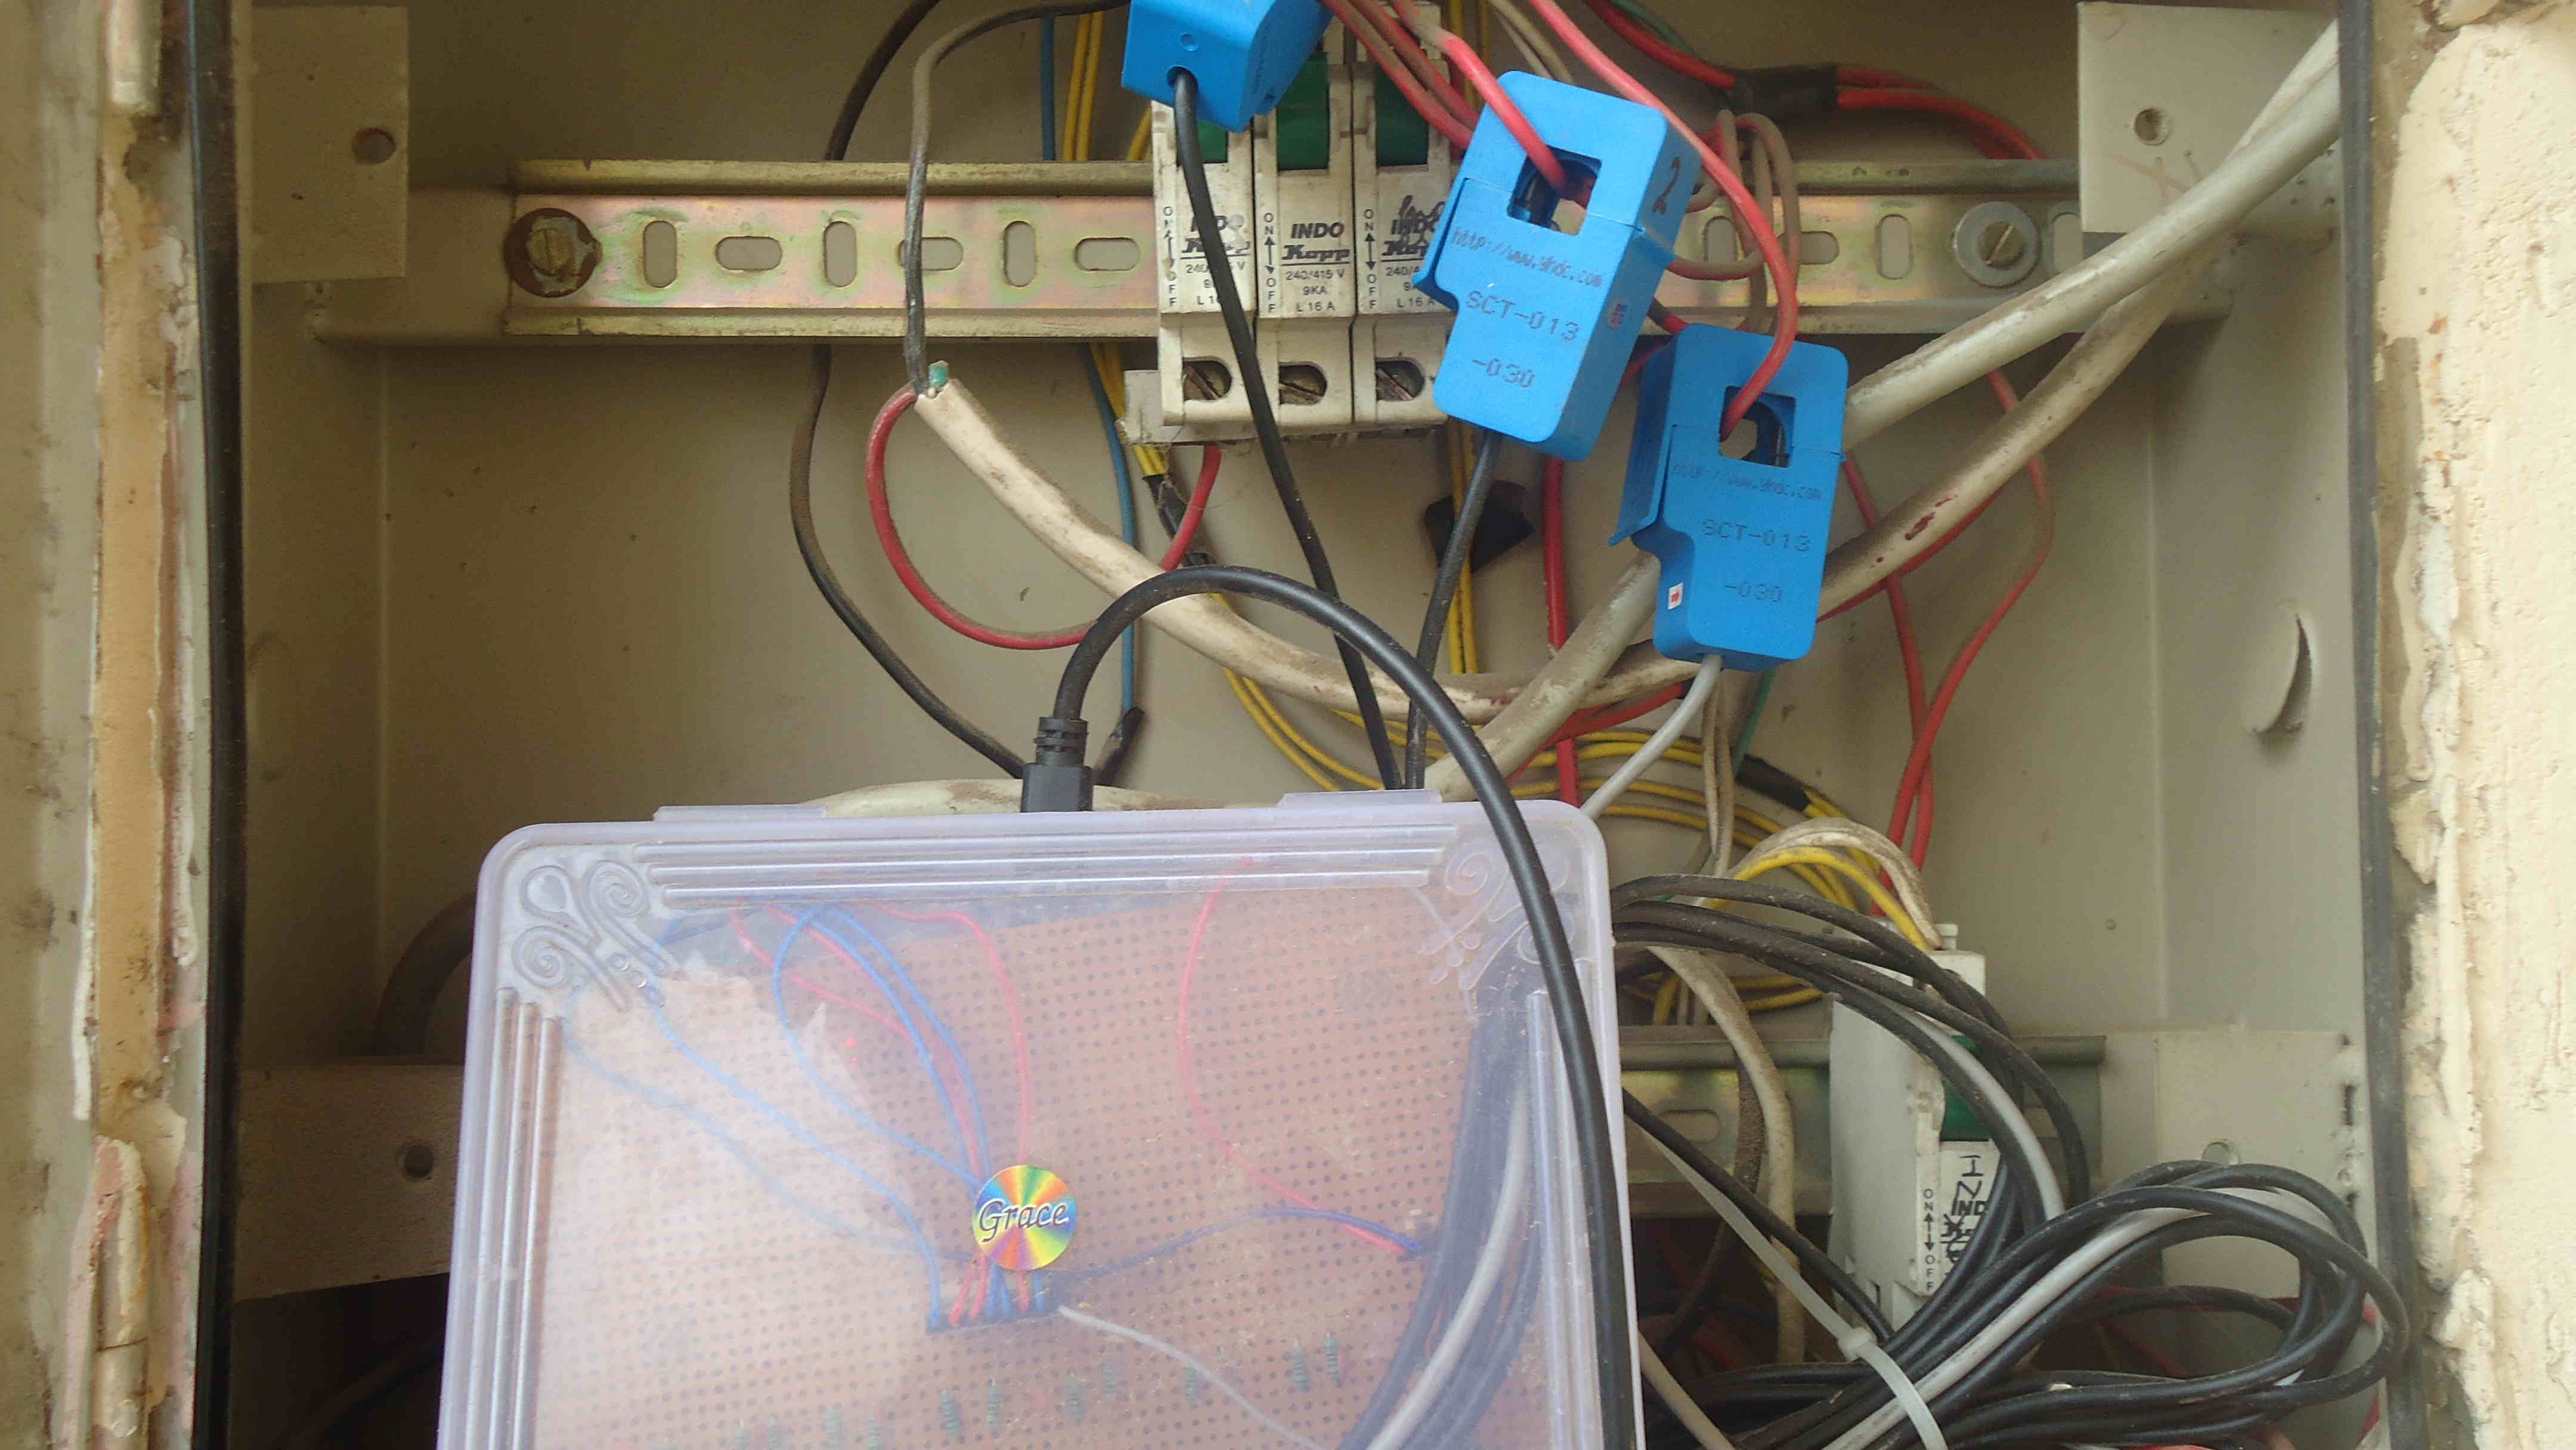
\includegraphics[scale=0.027]{./figures/mcb.jpg}}
       \hspace{1mm}
     \subfloat[\scriptsize Appliance level monitoring using jPlug]{
             \label{fig:jplug}
             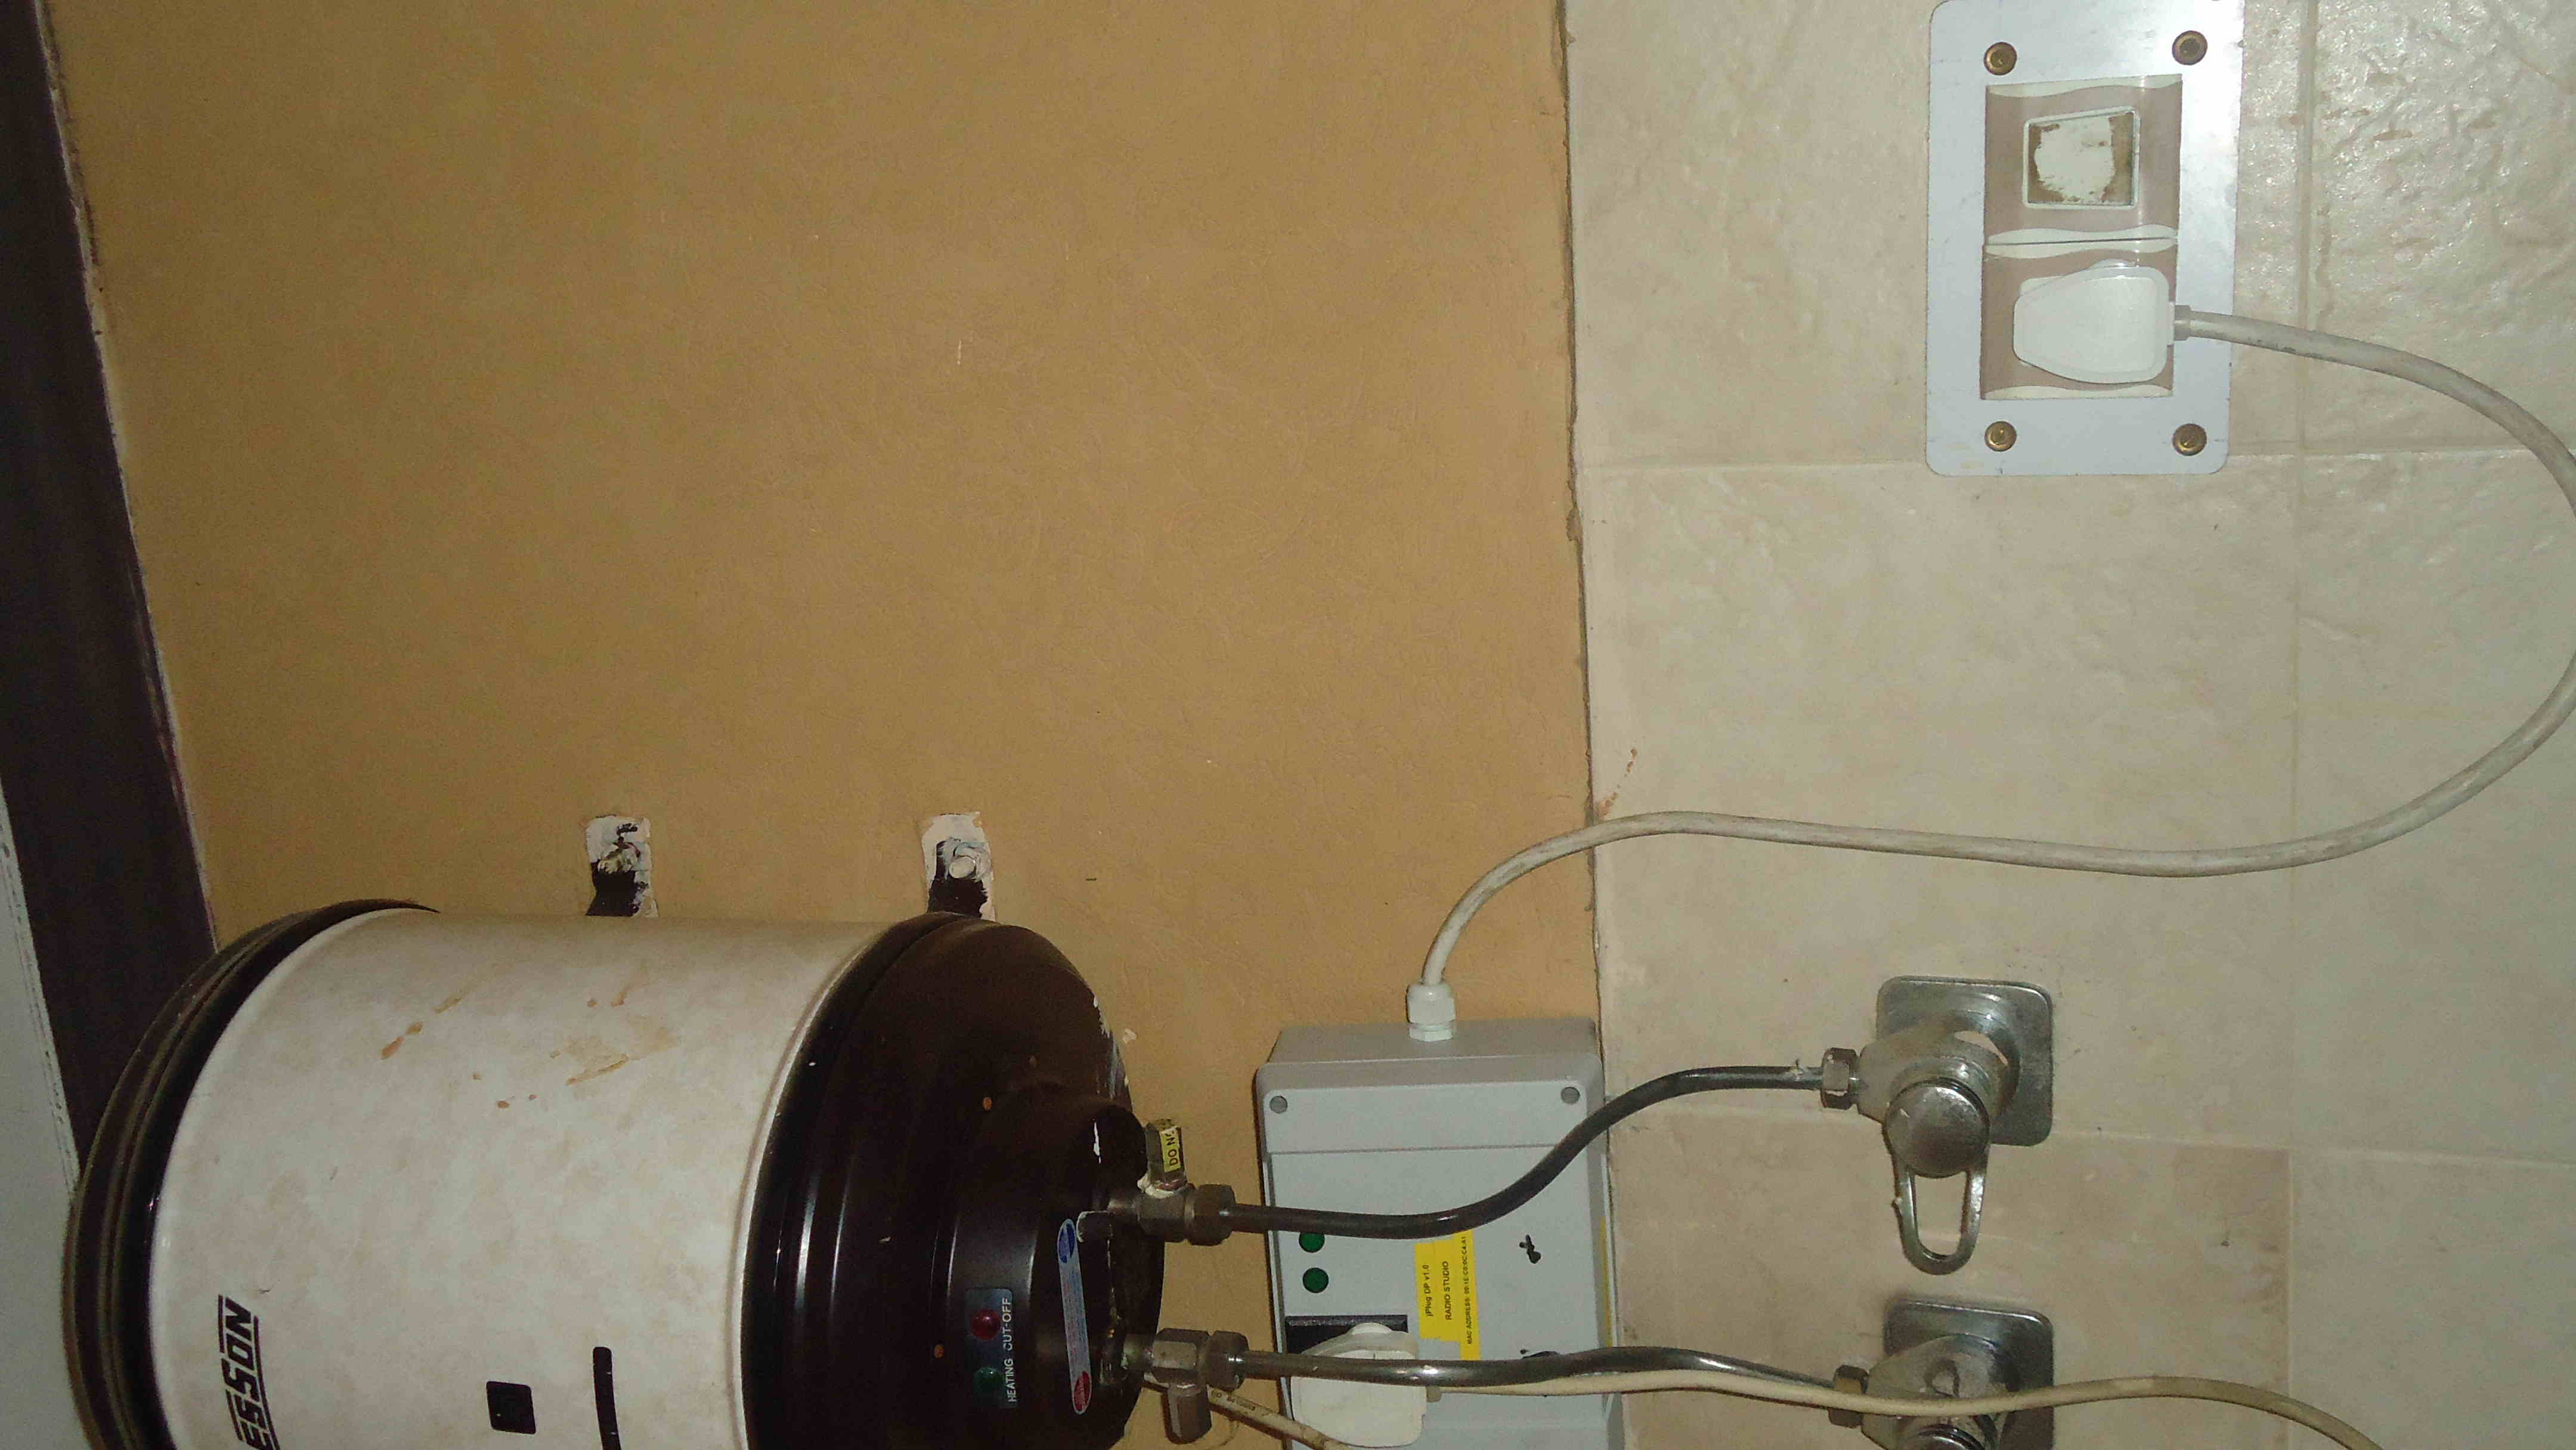
\includegraphics[scale=0.027]{./figures/jplug.jpg}}
             \hspace{1mm}
          \subfloat[\scriptsize Appliance level monitoring using Current Cost CT]{
                  \label{fig:cc}
                  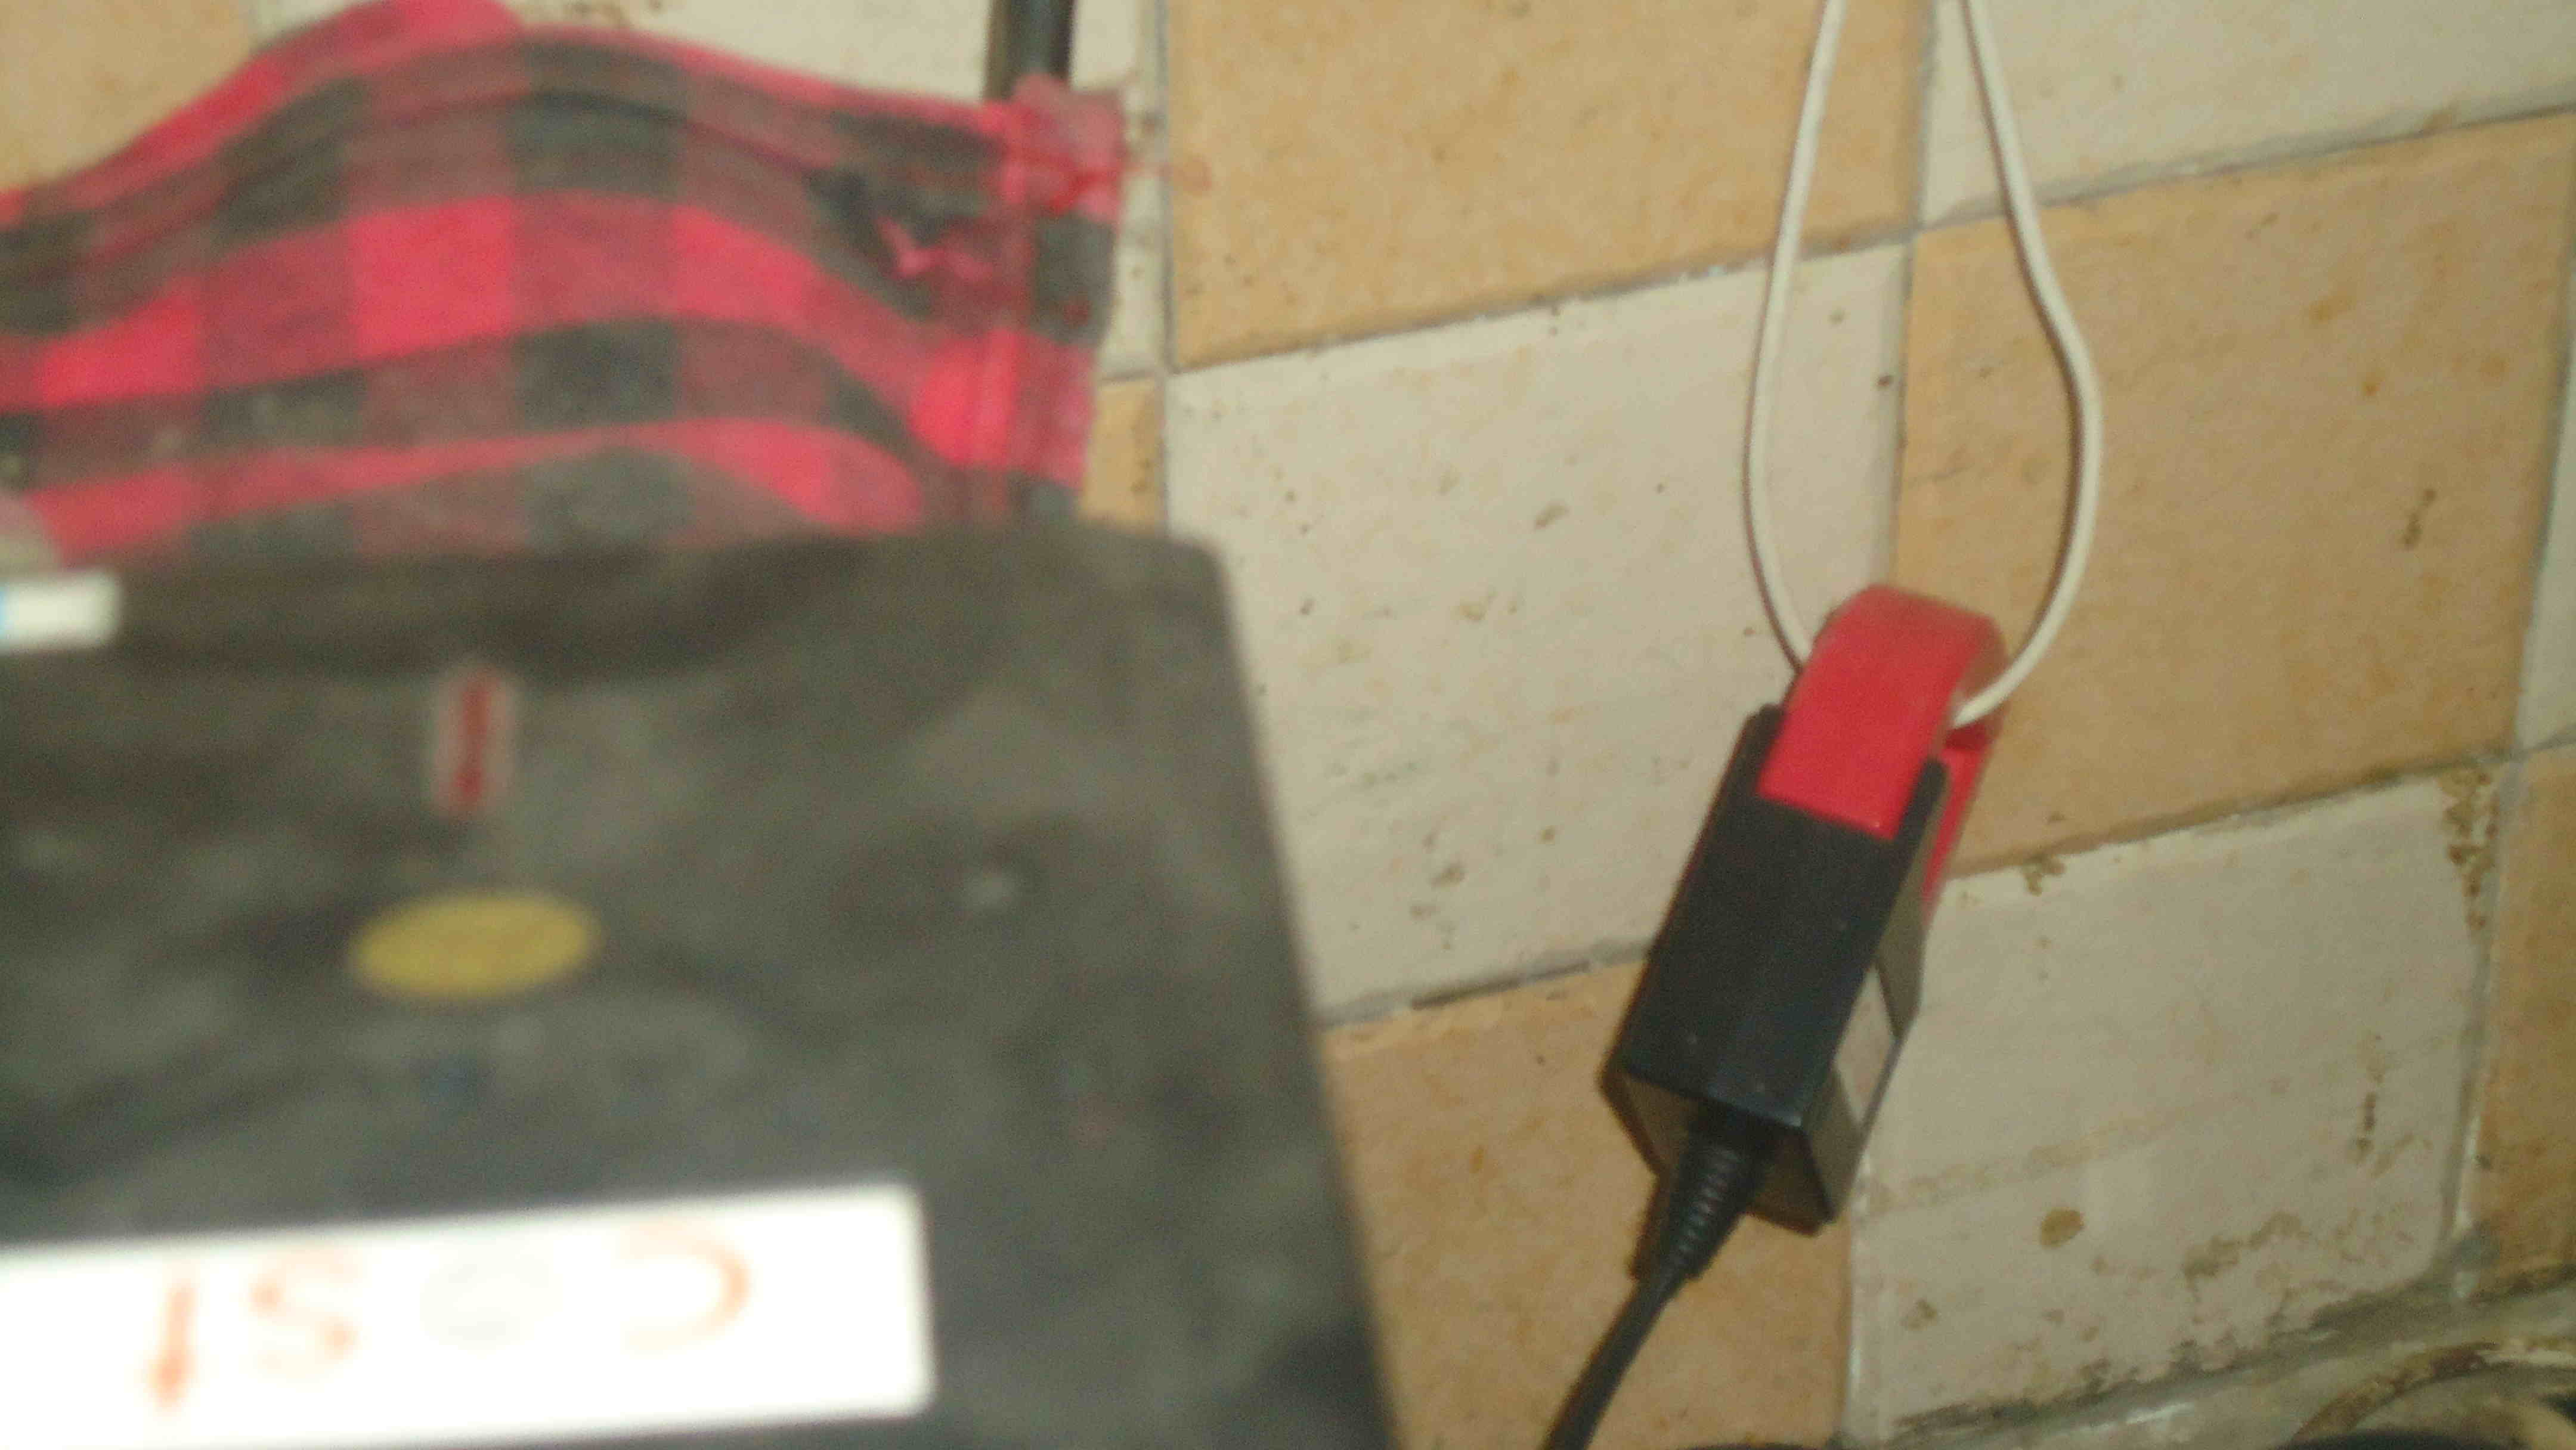
\includegraphics[scale=0.027]{./figures/cc.jpg}}
    %\hspace{0.02\columnwidth}
    \newline
    \vspace{-2mm}
    \subfloat[\scriptsize Water Meter]{
    \label{fig:water_meter}
        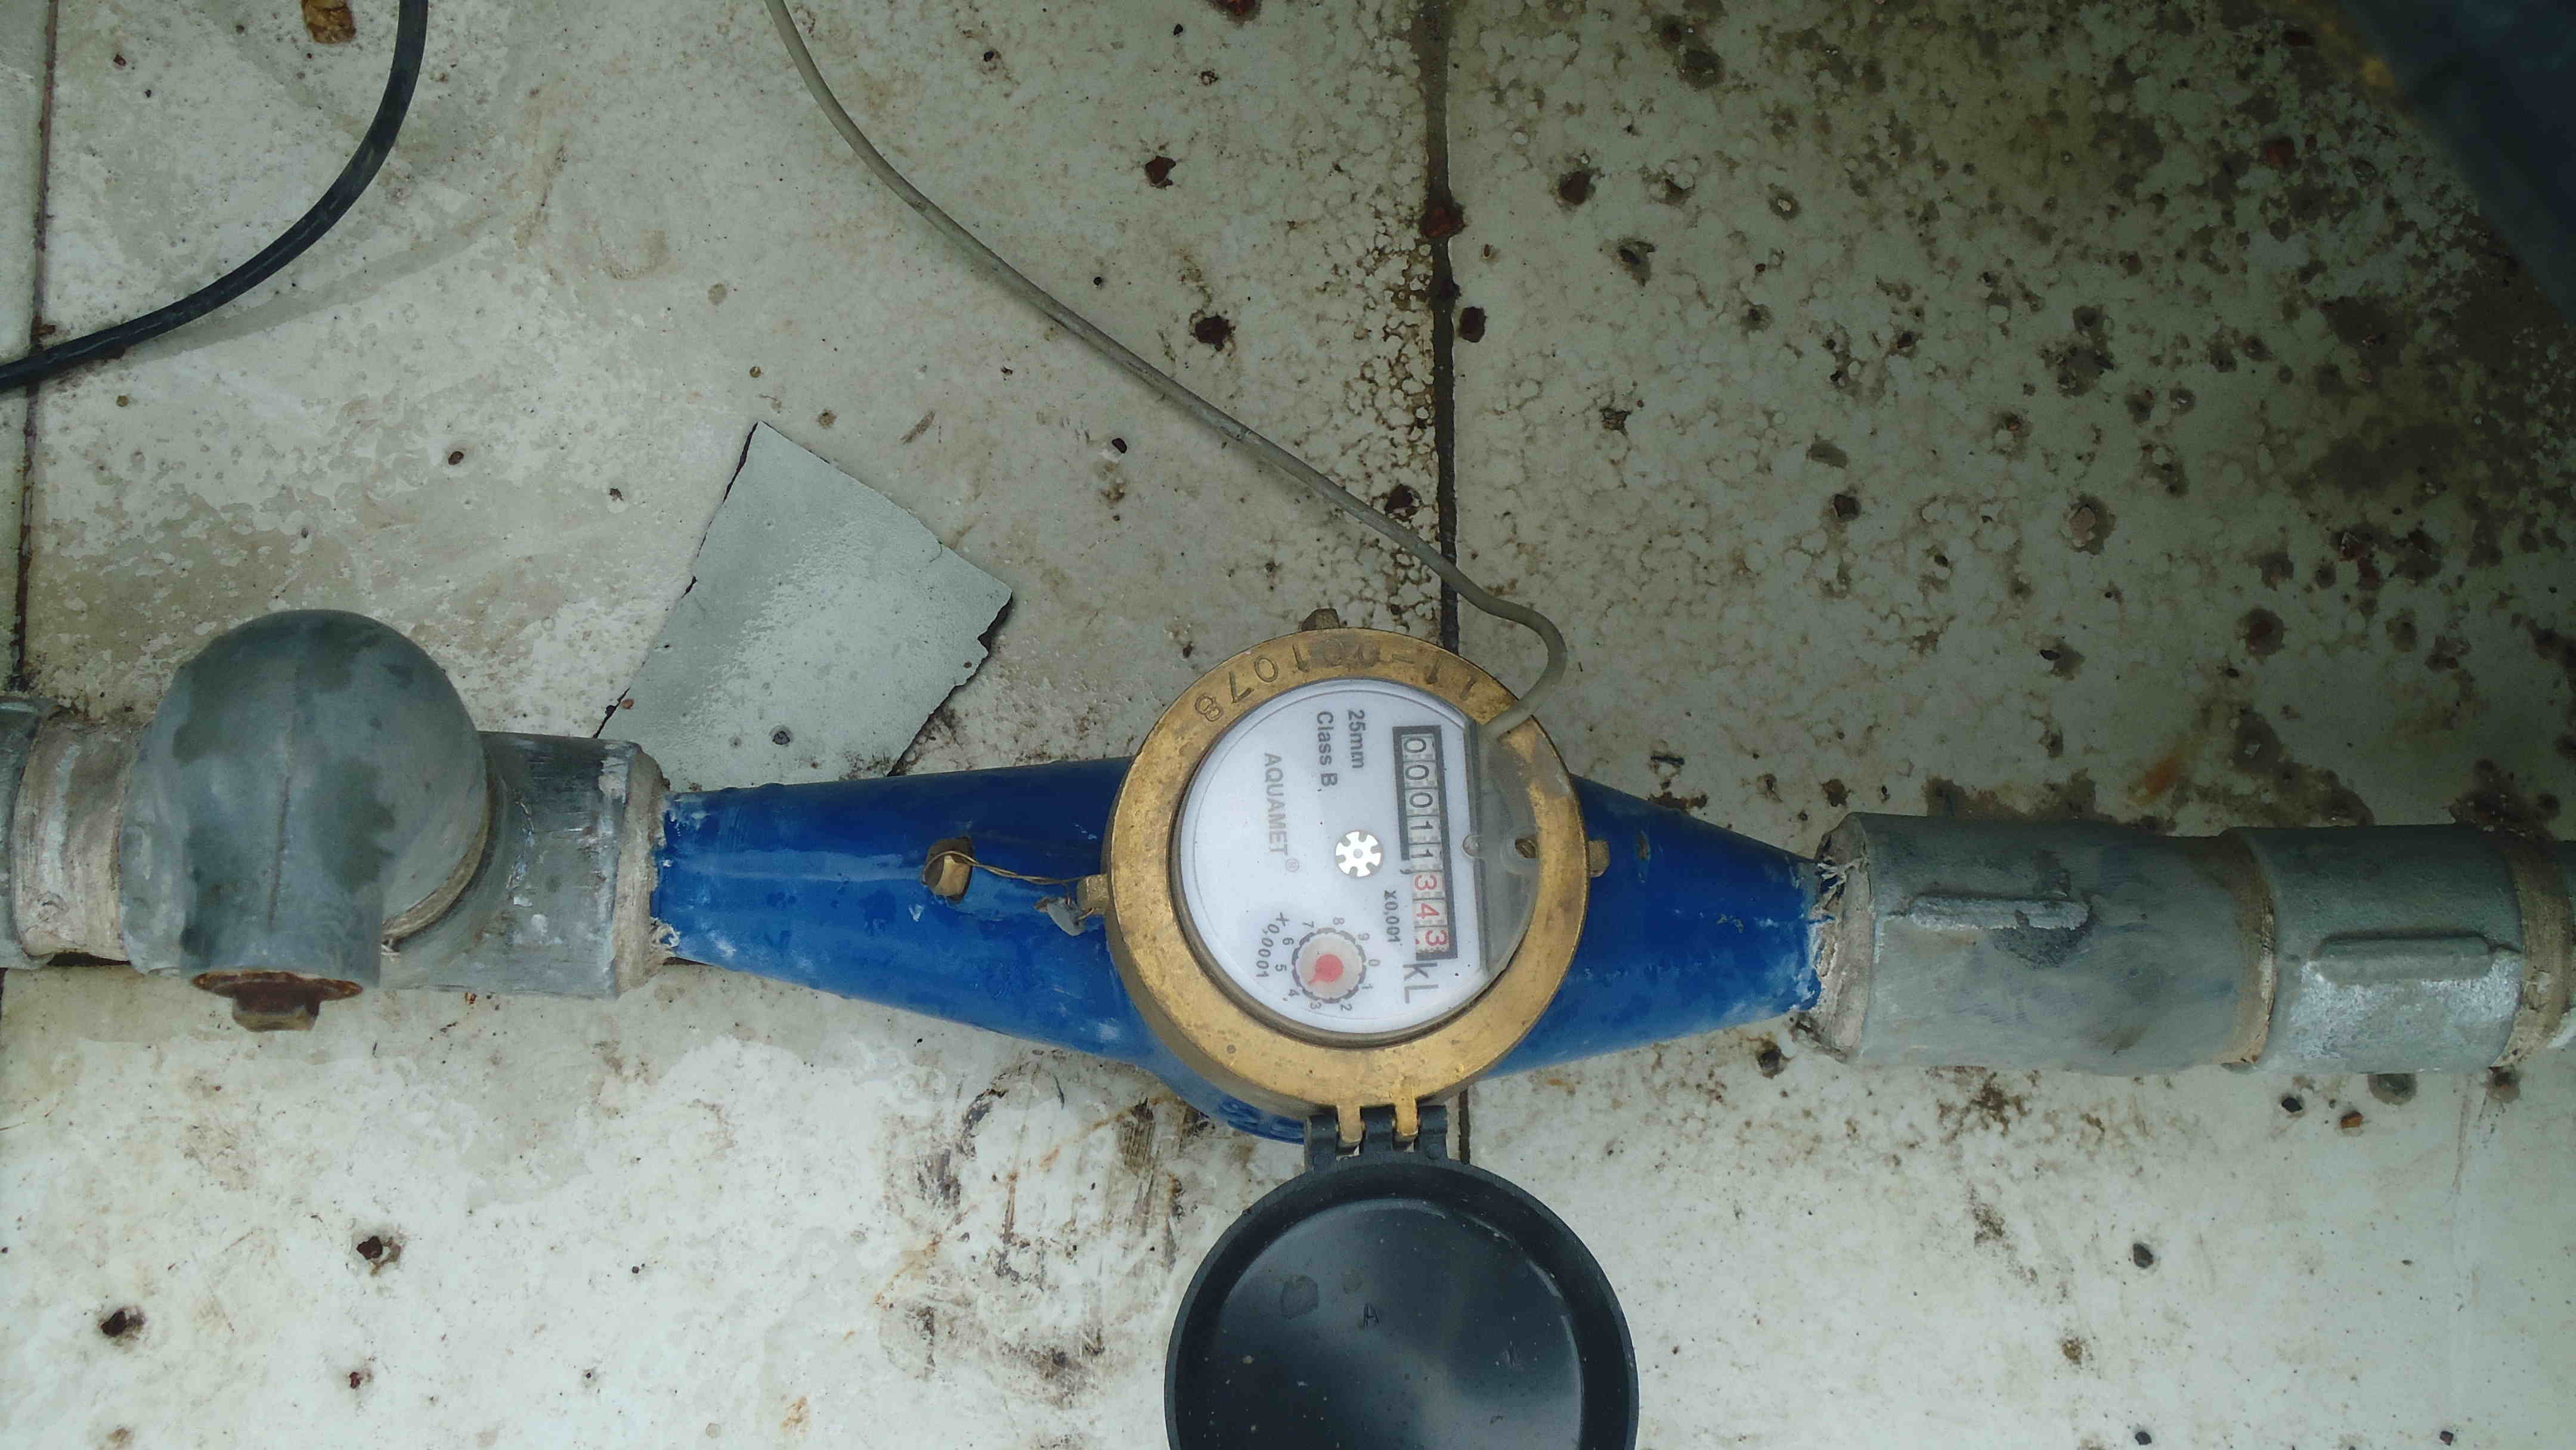
\includegraphics[scale=0.027]{./figures/water_meter.jpg}}
        \hspace{1mm}
     \subfloat[\scriptsize Android phone and Homeseer Zwave multisensor used to measure ambient parameters]{
        \label{fig:ambient}
            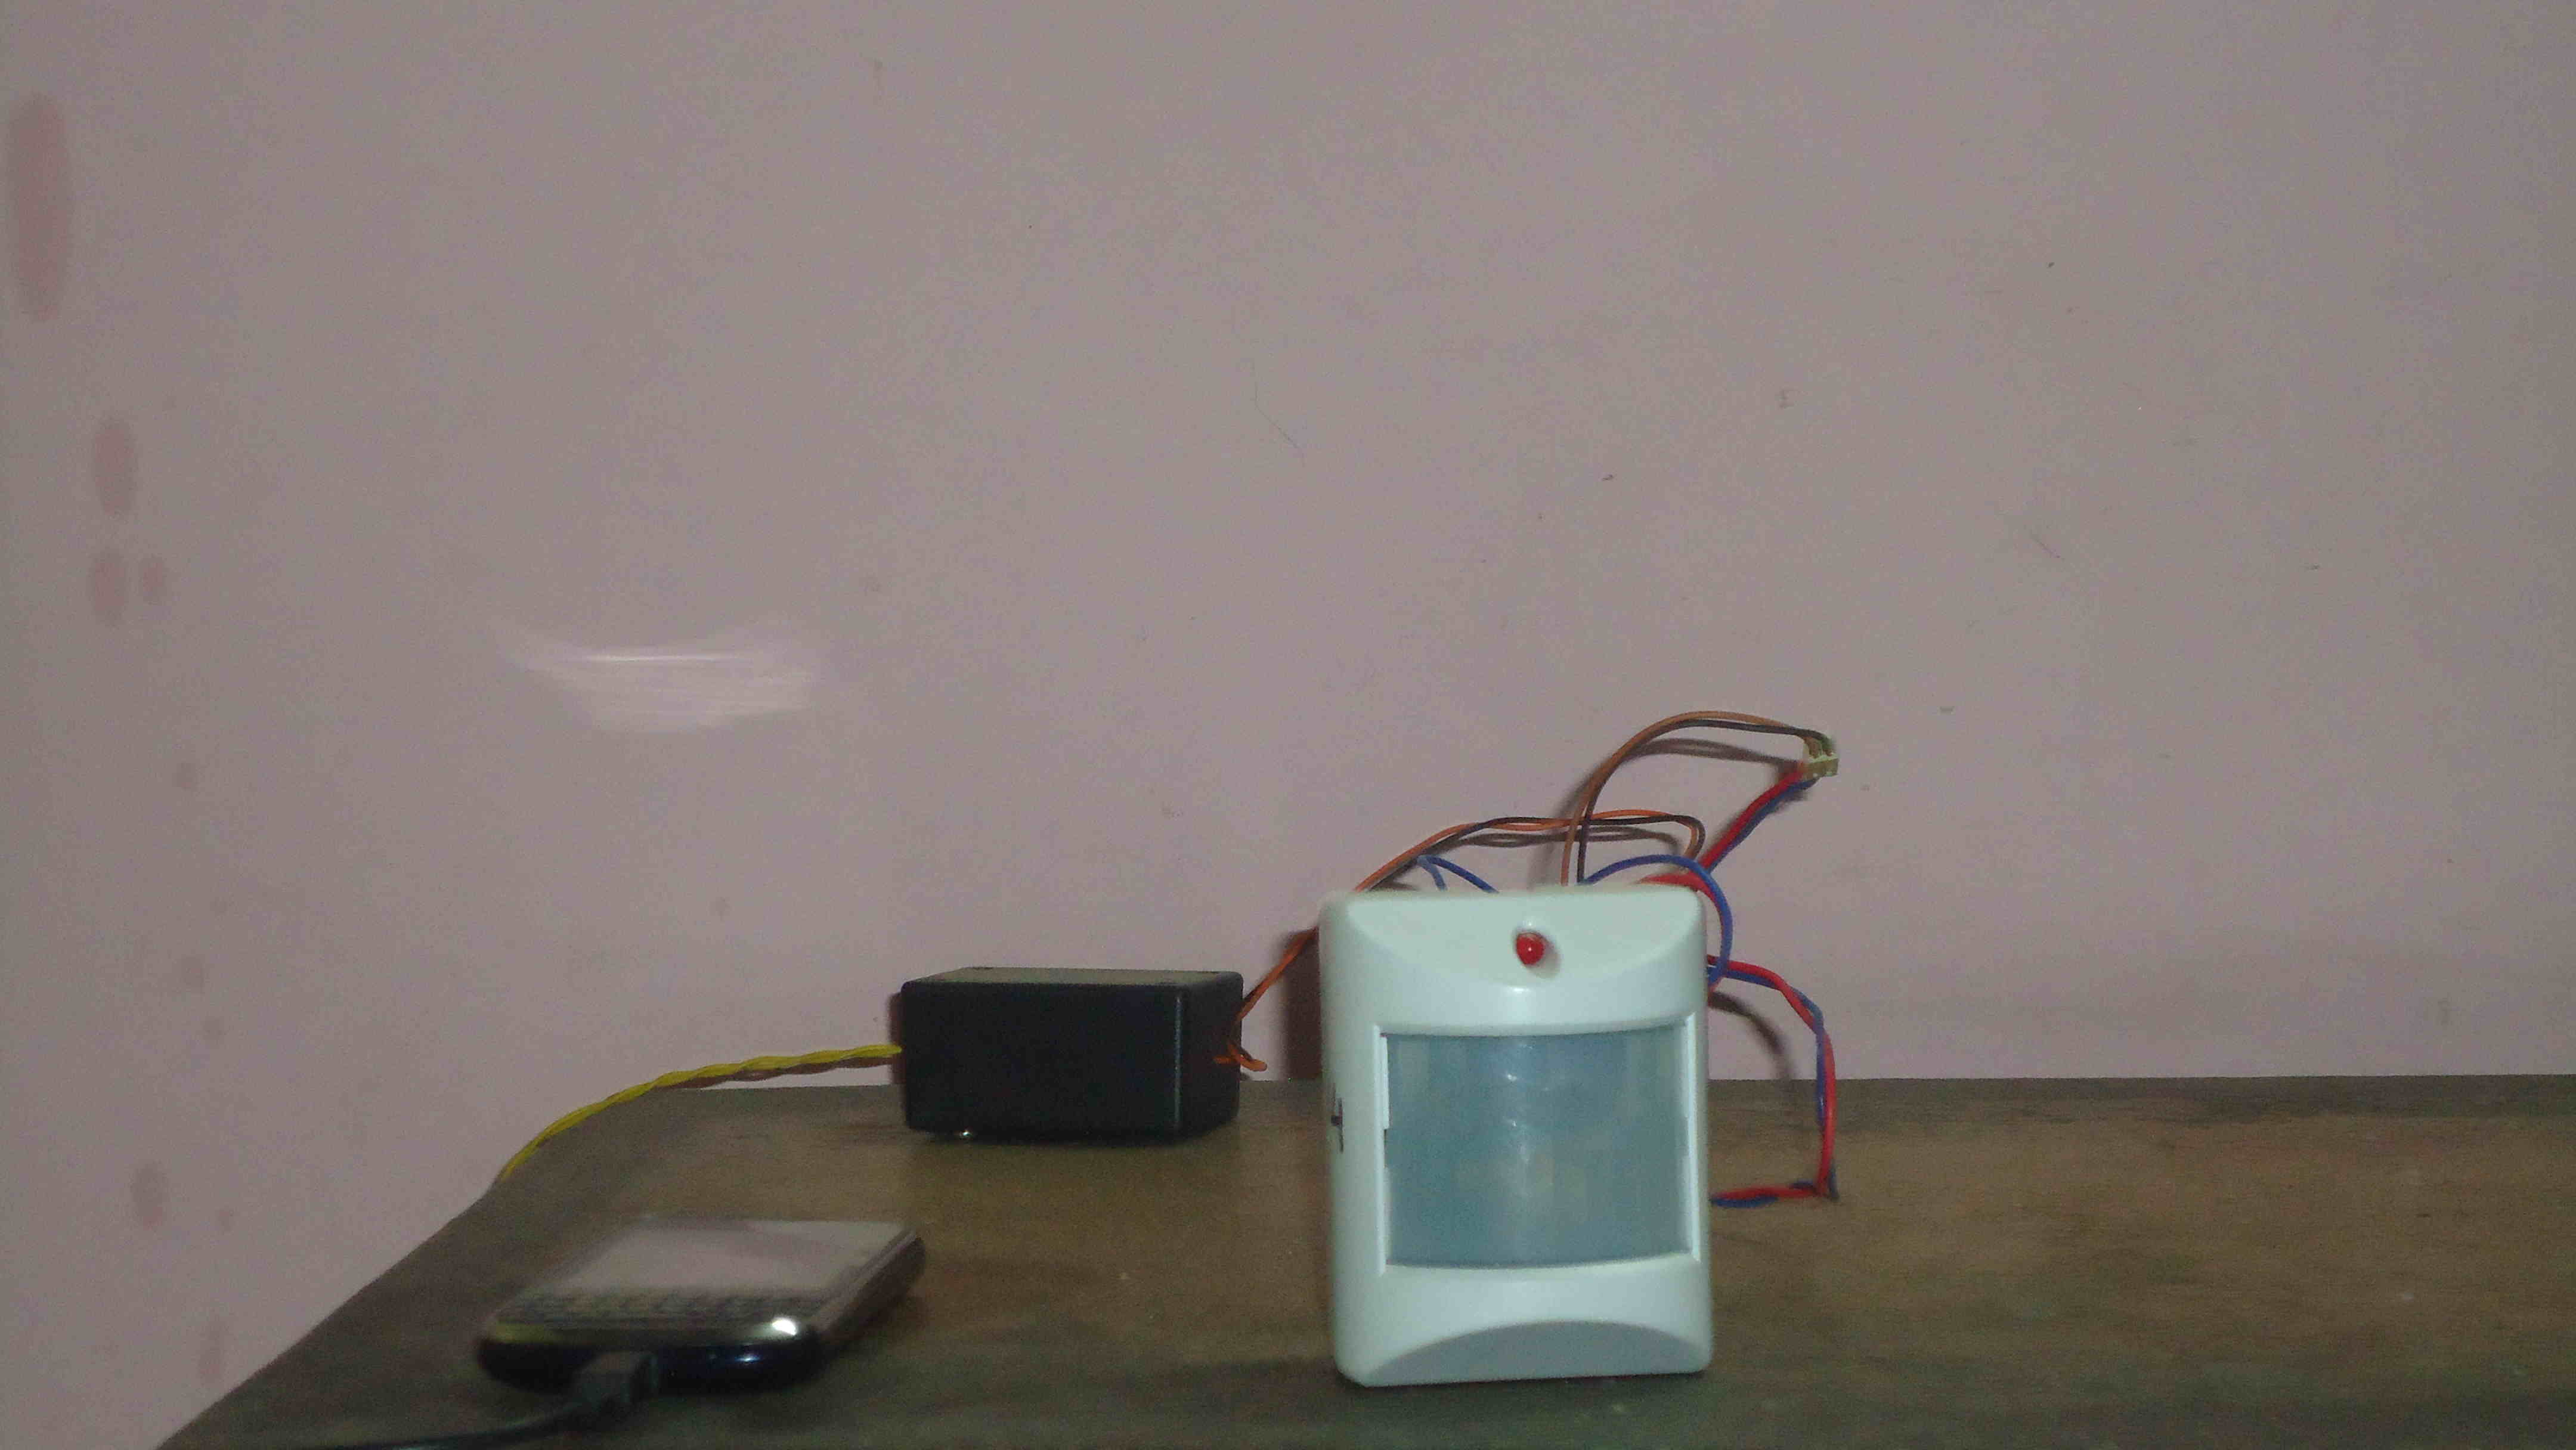
\includegraphics[scale=0.027]{./figures/ambient.jpg}}
            \hspace{1mm}
       \subfloat[\scriptsize Plug computer collecting data from ZWave controller and connected to the router via an ethernet cable]{
              \label{fig:plug}
                  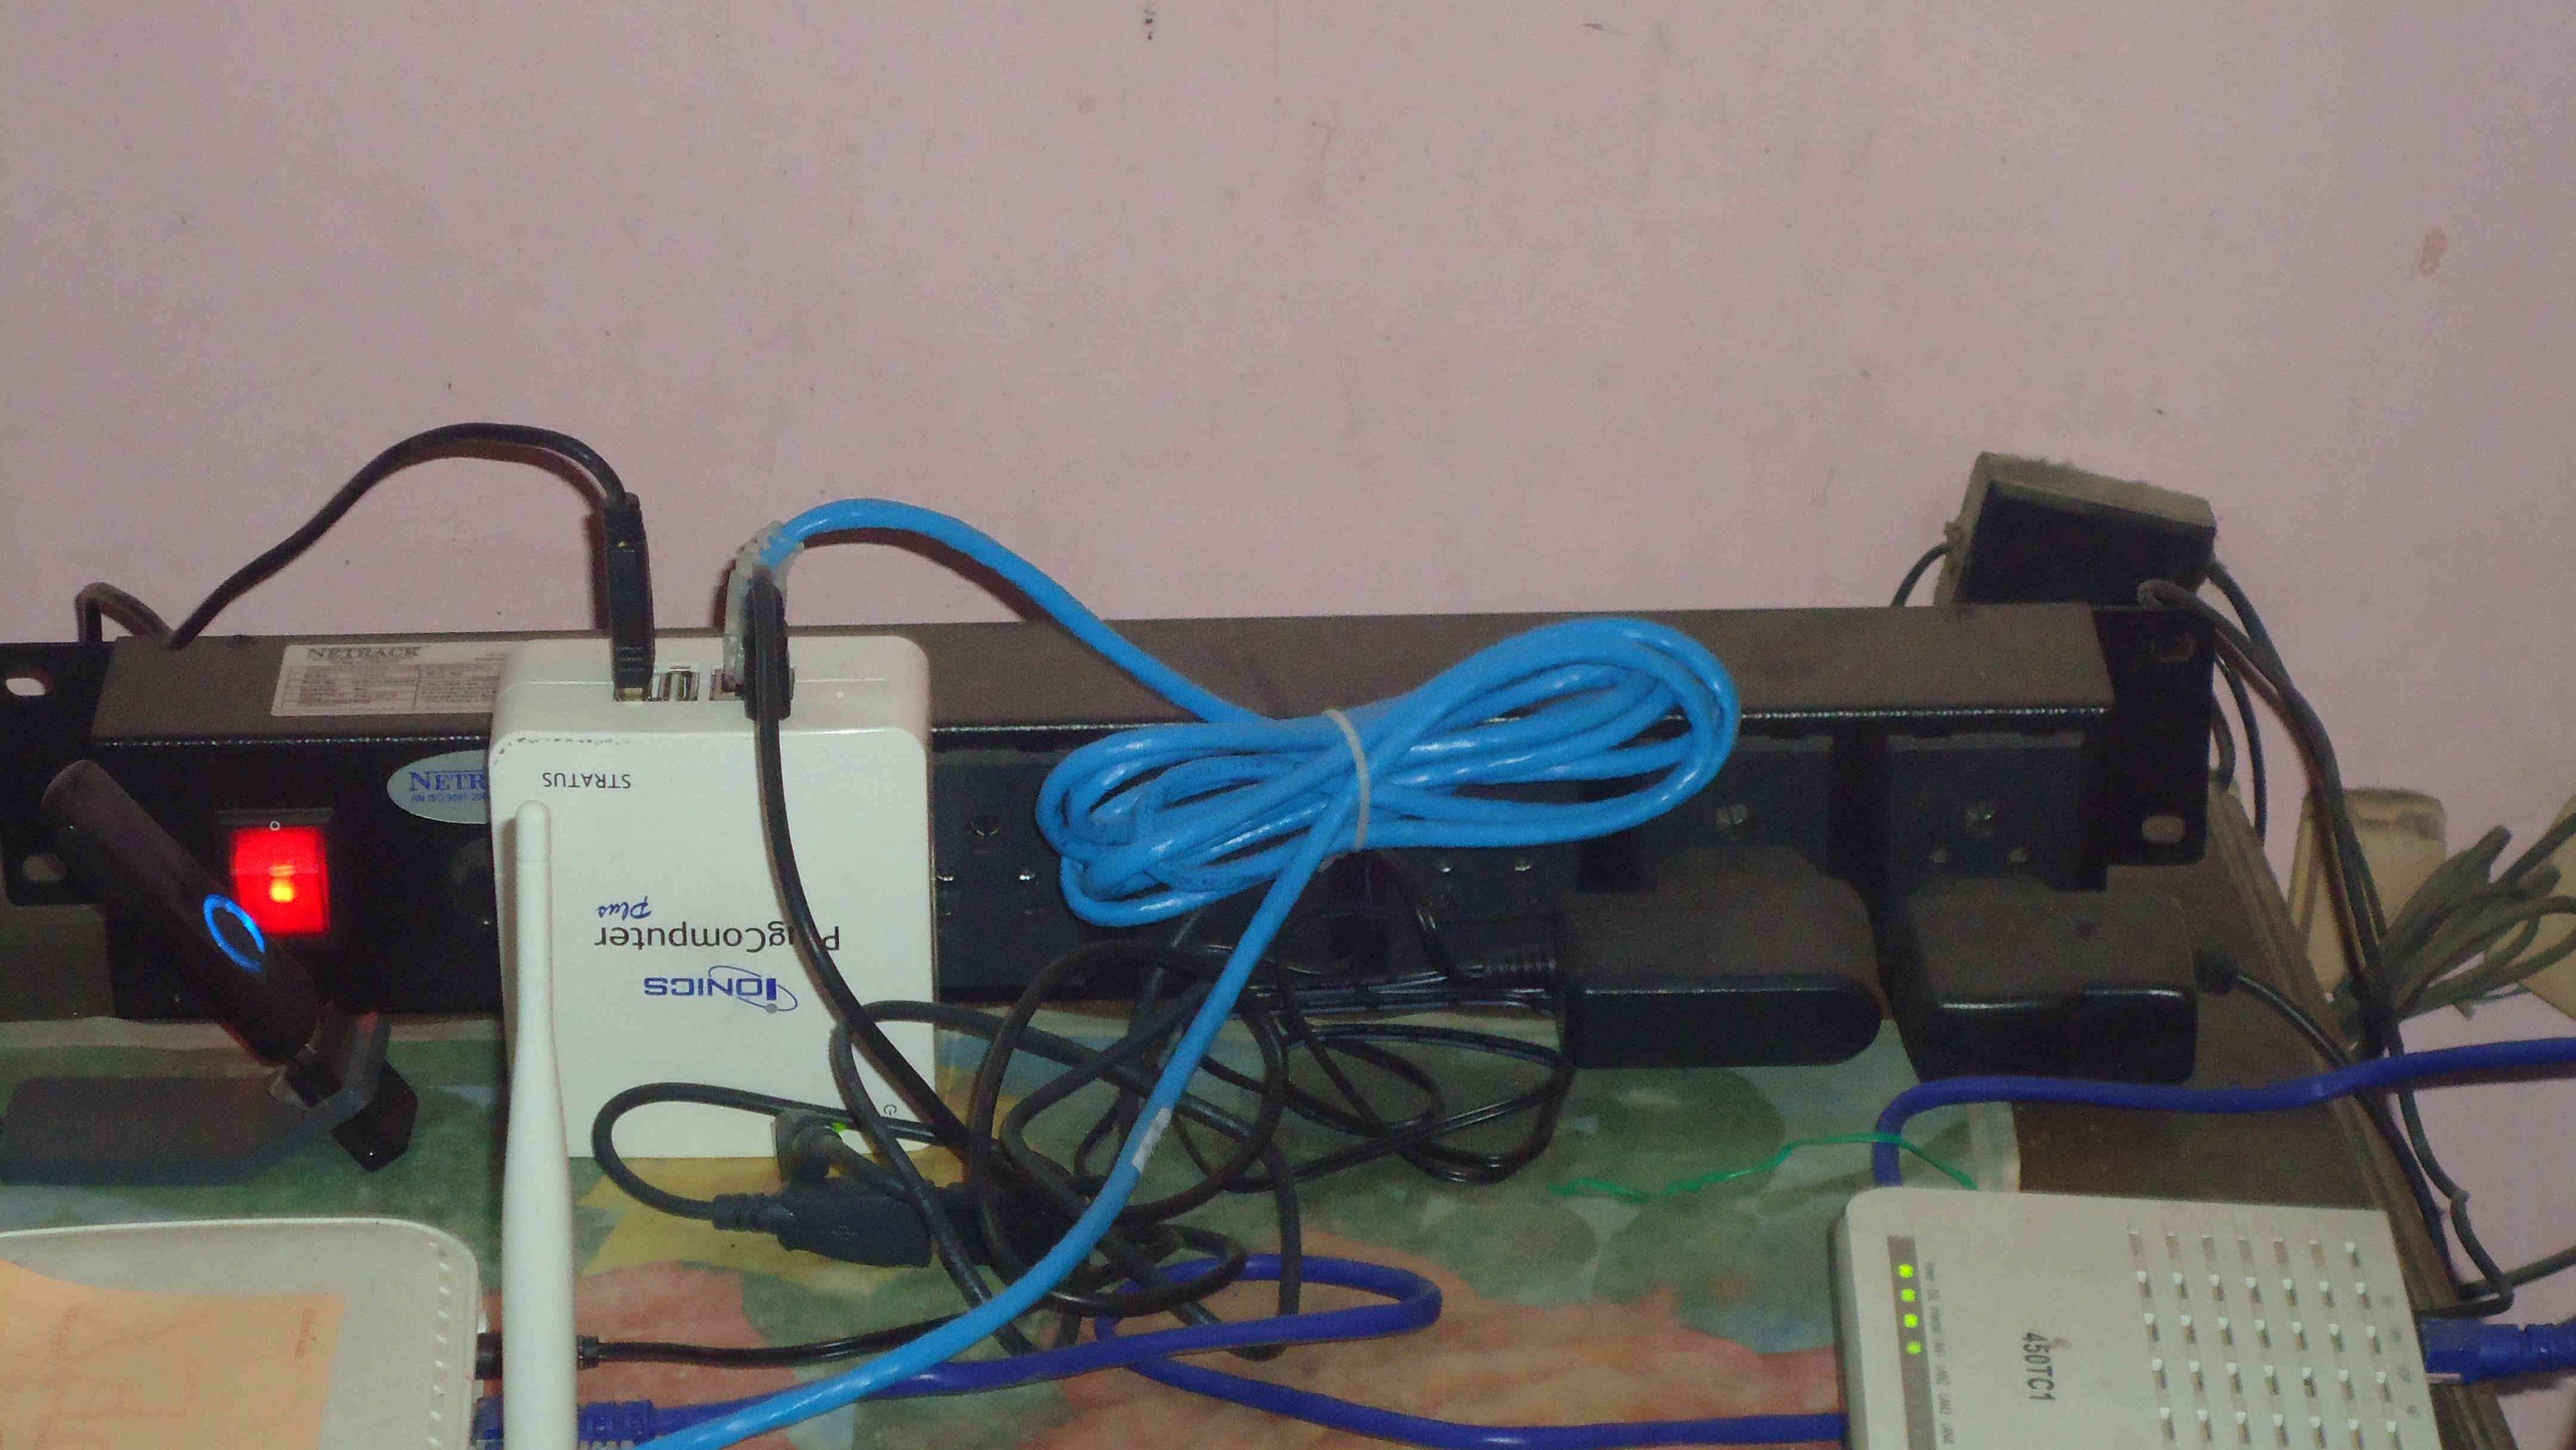
\includegraphics[scale=0.027]{./figures/plug.jpg}}
                  \hspace{1mm}
         \subfloat[\scriptsize RPi collecting water meter data using GPIO pins]{
                     \label{fig:rpi}
                         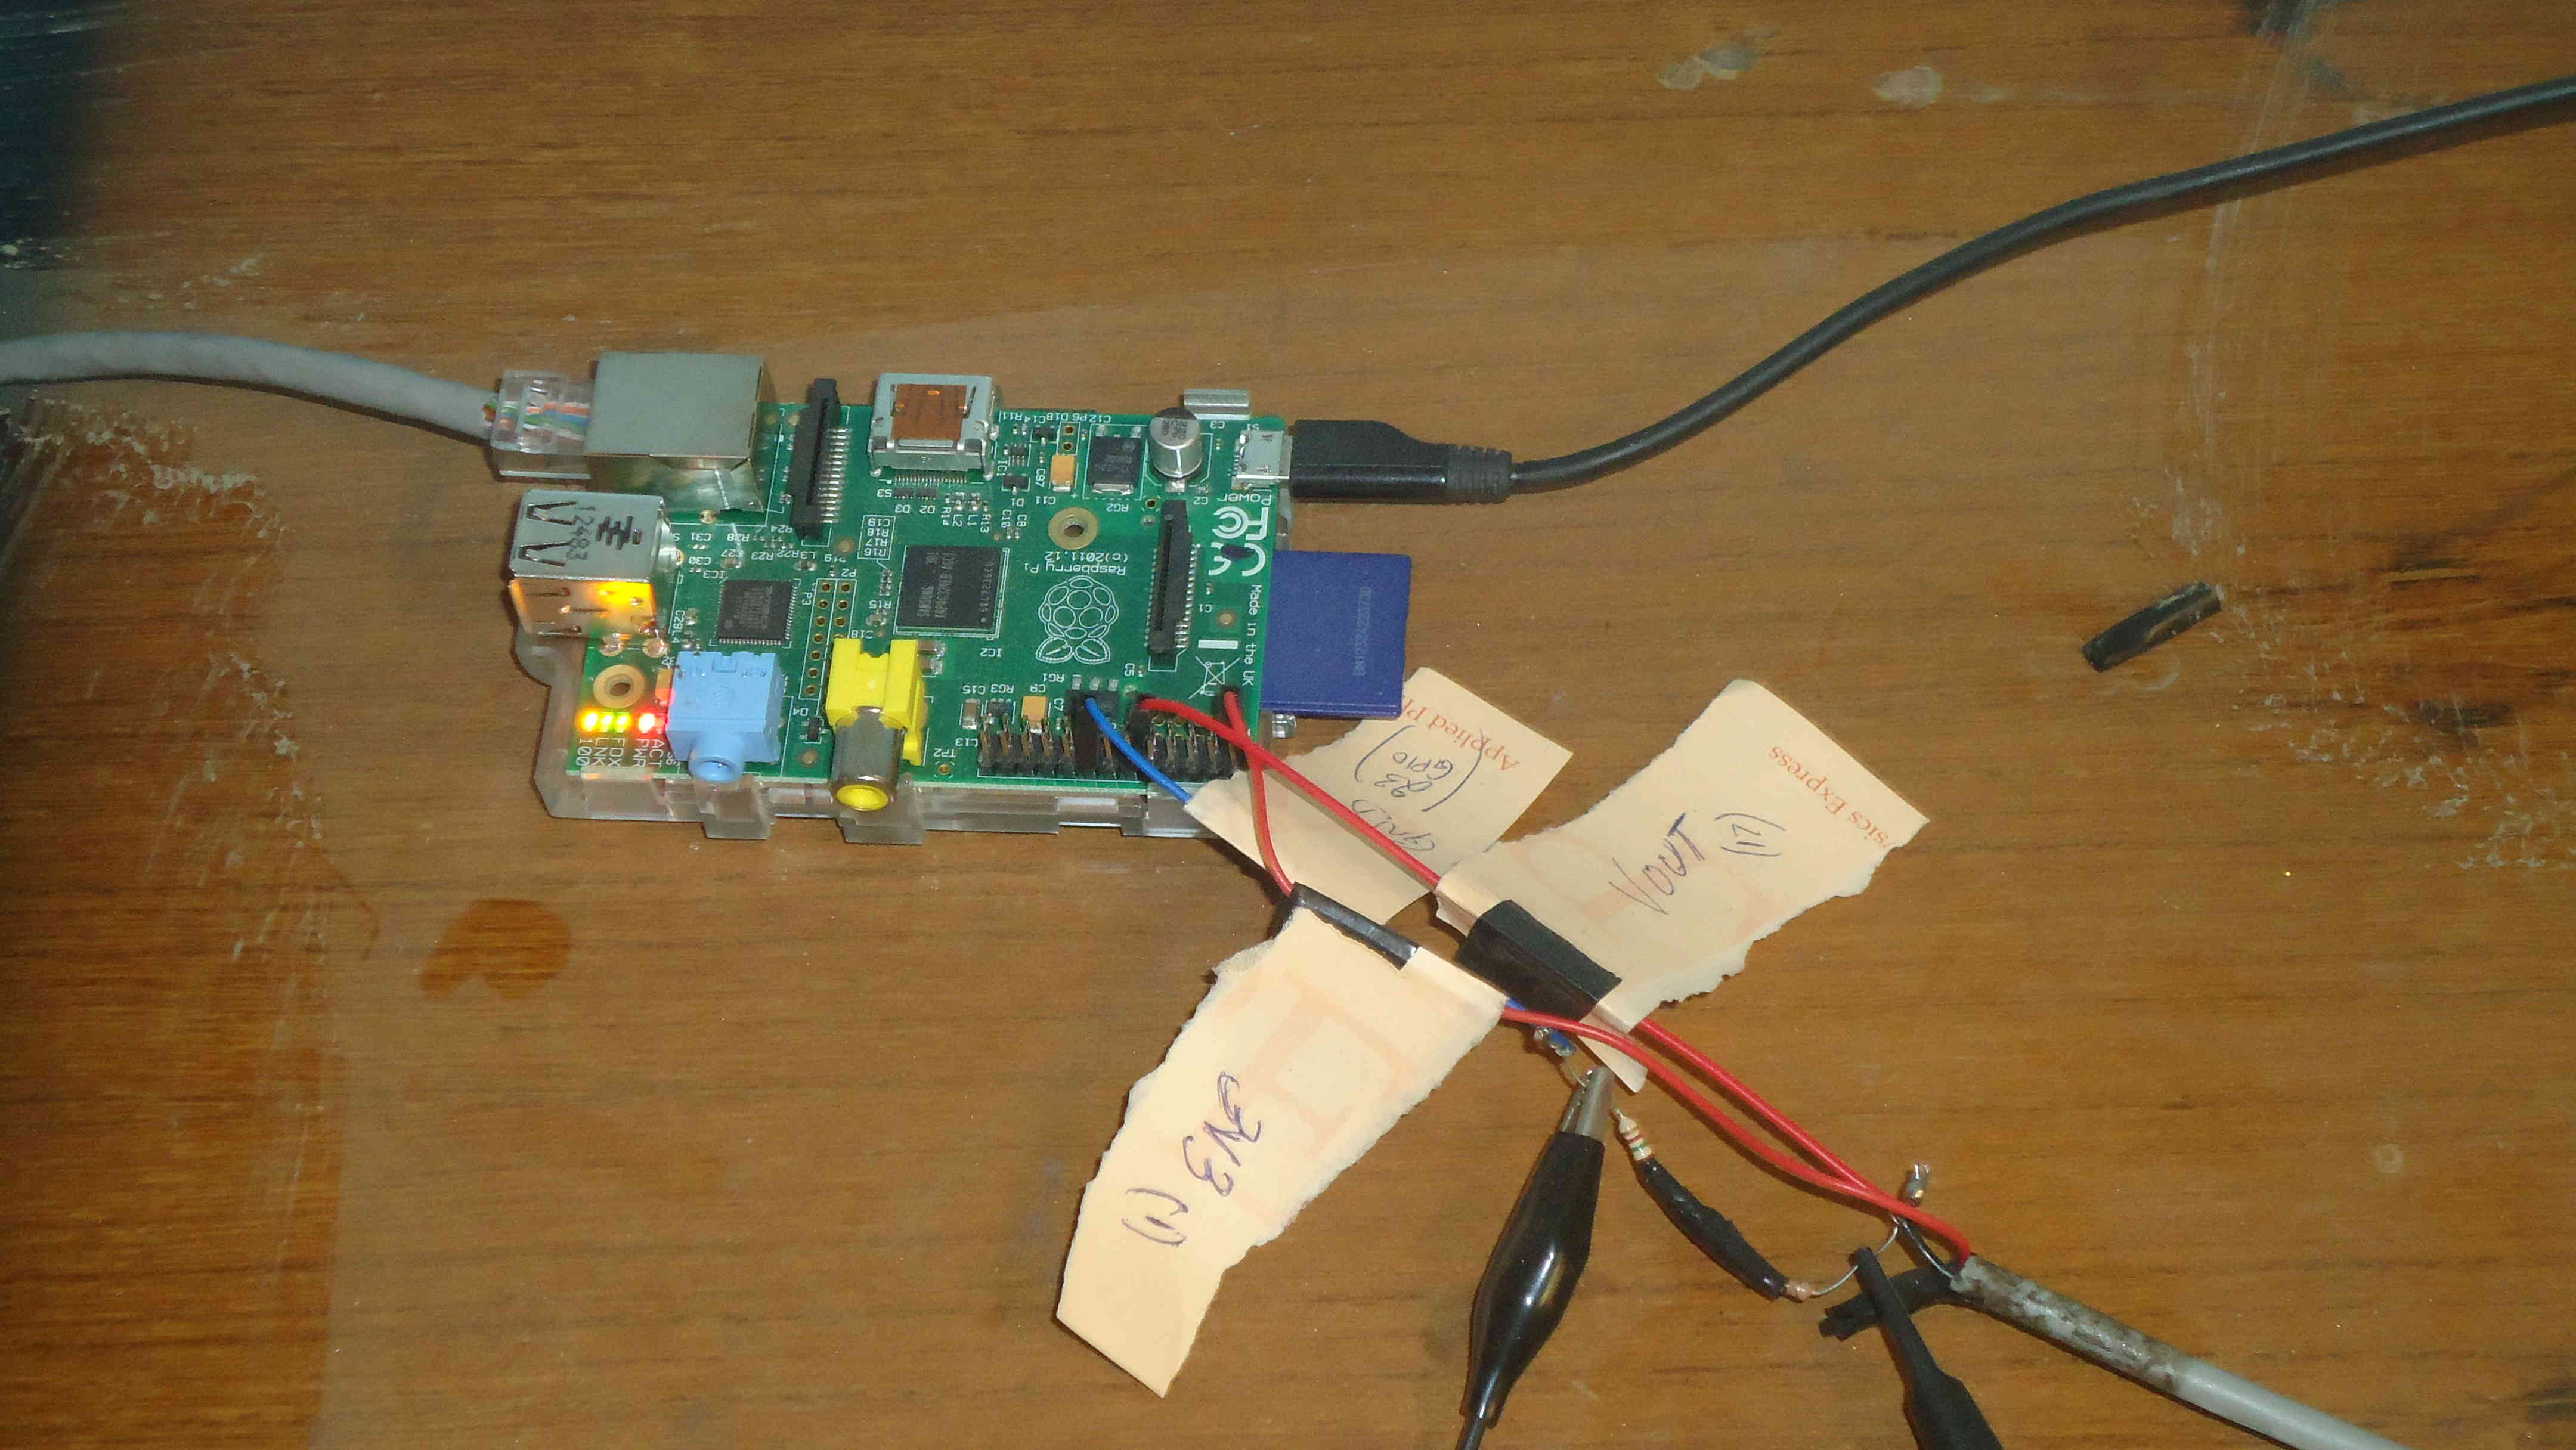
\includegraphics[scale=0.027]{./figures/rpi.jpg}}

    \caption{Sensing, computation and communication equipment used for deployment}

    \label{fig:deployment}

\end{figure*}

\section{How is this deployment different?}
\label{sec:learning}
In this section we discuss unique aspects brought forward from our deployment. Some of the key aspects are as follows:
\begin{itemize}

\item \textbf{Unreliable grid is commonplace:} Load shedding or rolling blackout are common in developing countries, owing to several reasons such as improper infrastructure management, high demand and low electricity production. Power cuts are more common in summers when load is higher due to usage of air conditioners. As a result, voltage fluctuations are also common. Previous work \cite{nplug} has hypothesized that frequency and voltage indicate load on the grid. 
for electricity number of hours failure, failure by n'th hour, hist of failure hours
\item Homes have poor connectivity. This forced us to develop a different paradigm which we call Sense-Store-Transfer. This is shown in \figref{fig:network}

\item \textbf{Importance of meta data collection:}

\begin{figure}
\subfloat[\scriptsize Before repair]{
    \label{fig:before_repair}
    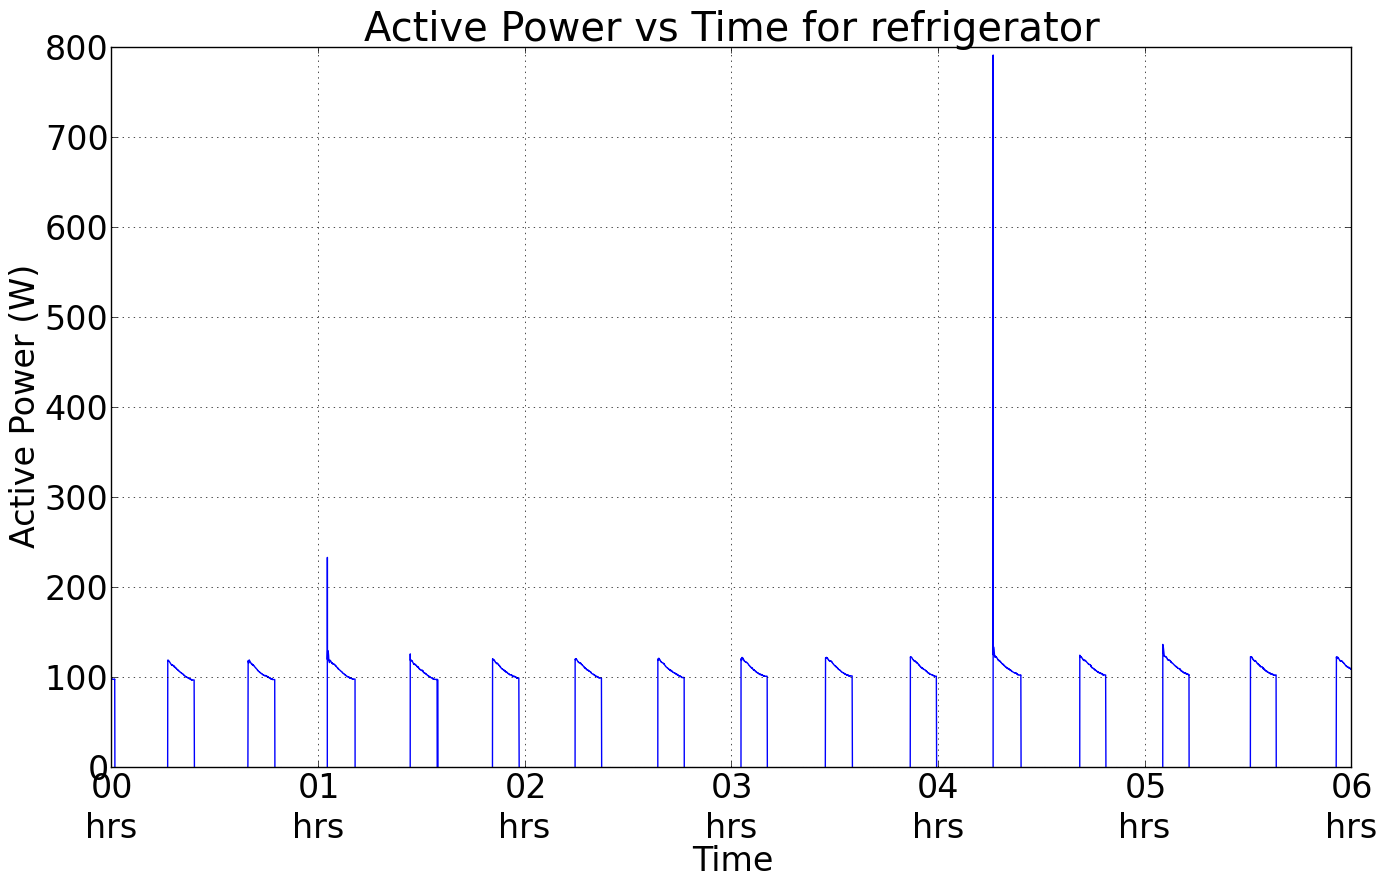
\includegraphics[scale=0.13]{./figures/before_repair.png}}
     \subfloat[\scriptsize Electricity failure durations ]{
        \label{fig:after_repair}
        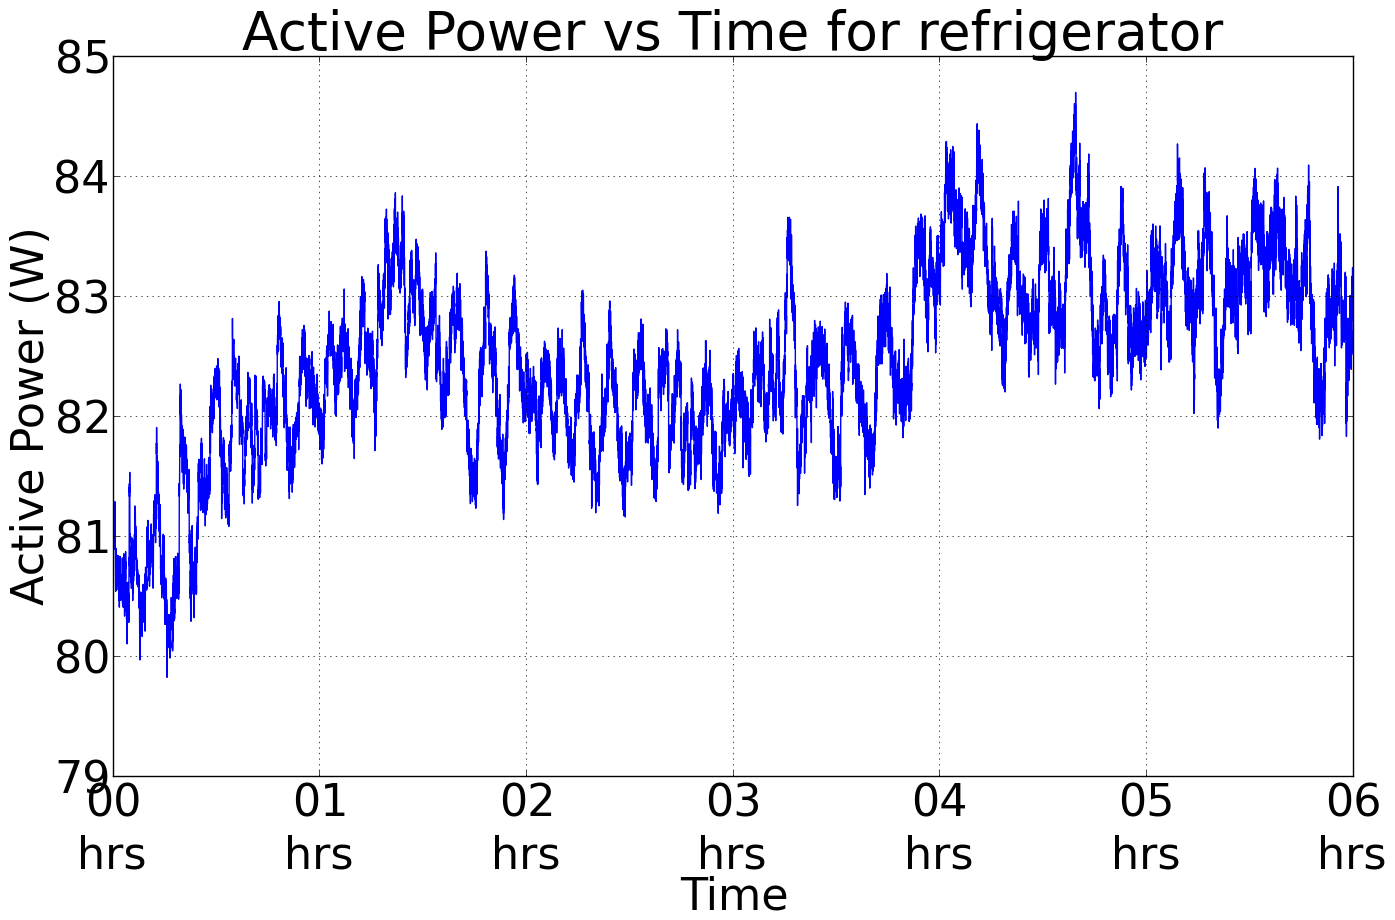
\includegraphics[scale=0.13]{./figures/after_repair.png}}
       
   
    \caption{Refrigerator power consumption}

    \label{fig:metadata}

\end{figure}

\item Homes are hazardous environments
\begin{itemize}
\item Multi failed when put on inverter point
\item Node in one room will always fail
\item Wire snag and how it led to data loss of node 4
\end{itemize}

\item Homes are remote environments:
We had to raise ~60 new issues on Github. We first did deployment in researchers home which had full access to all nodes.
We also provided alerting mechanisms.

\item User participation
Even at researchers home, had asked the researcher to take notes. But even his engagement was not 100 \%.

\item Aesthetics matter
\begin{itemize}
\item LED in night \figref{fig:led}
\item Noise- Noisy SMPS due to dust. Unique to our setting. Figure from FunF showing sound level before and after cleaning.
\end{itemize}

\item Simplify the architecture
We used Load-Store-Forward. Describe this in more detail and relate to earlier n/w connectivity.
Also when number of systems is so large, simple CSV uploading is the best mechanism.

Wherever possible use Ethernet with repeaters. Also, RPi are known to have problems with WiFi.

\item Importance of meta data and calibration
Figure showing power consumption of ref. after repair
Figure showing different measurements for same appliance
Figure showing voltage fluctuations

\item Provision for more sensors than actual number required. x jplug, y multisensor failed due to ..
\item Non availability of sensors in local markets

\end{itemize}
\begin{figure*} 
    
    \subfloat[\scriptsize Electricity failure vs Time]{
    \label{fig:failure_time}
    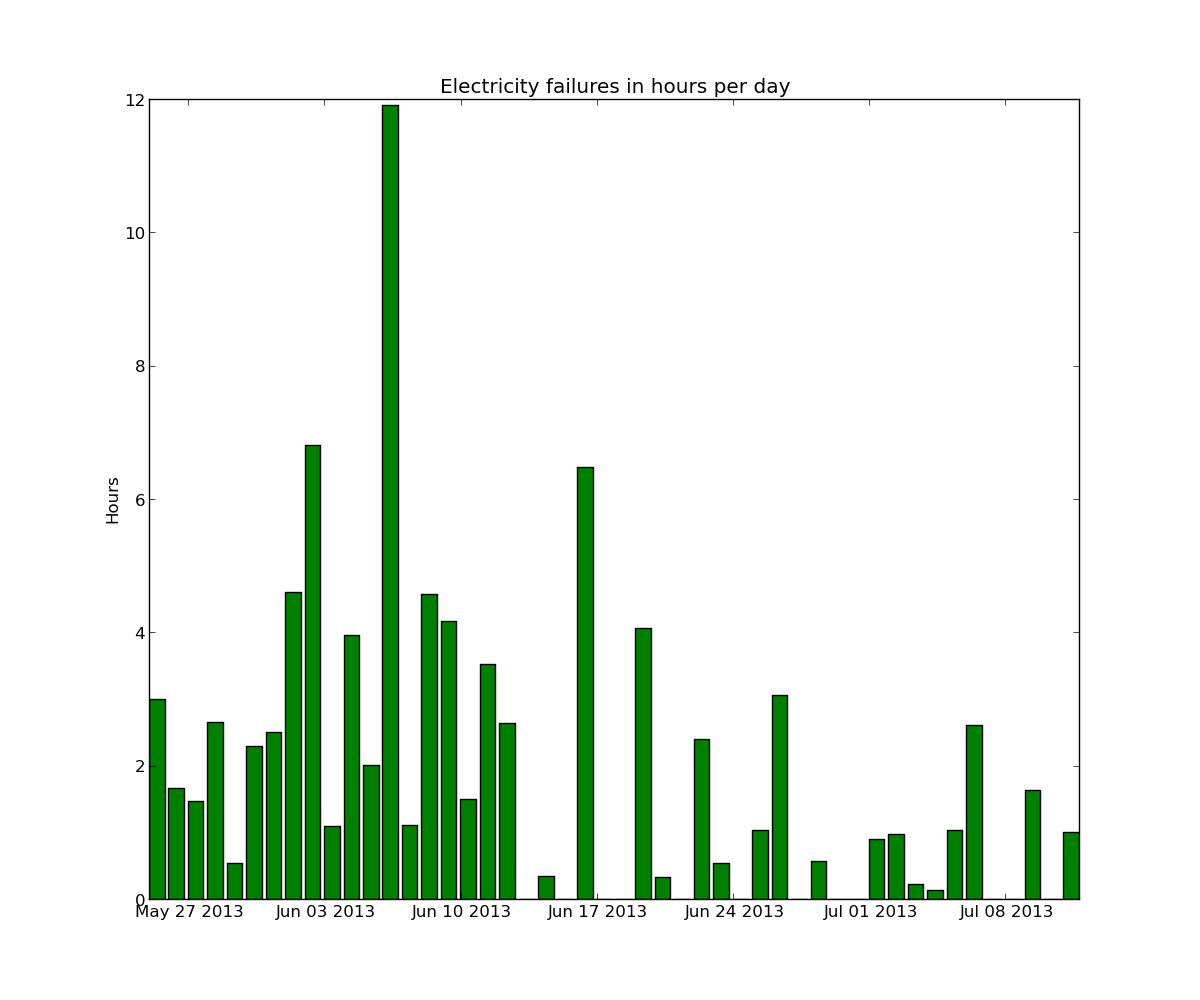
\includegraphics[scale=0.15]{./figures/electricity.png}}
    \hspace{1mm}
     \subfloat[\scriptsize Electricity failure durations ]{
        \label{fig:failure_duration}
        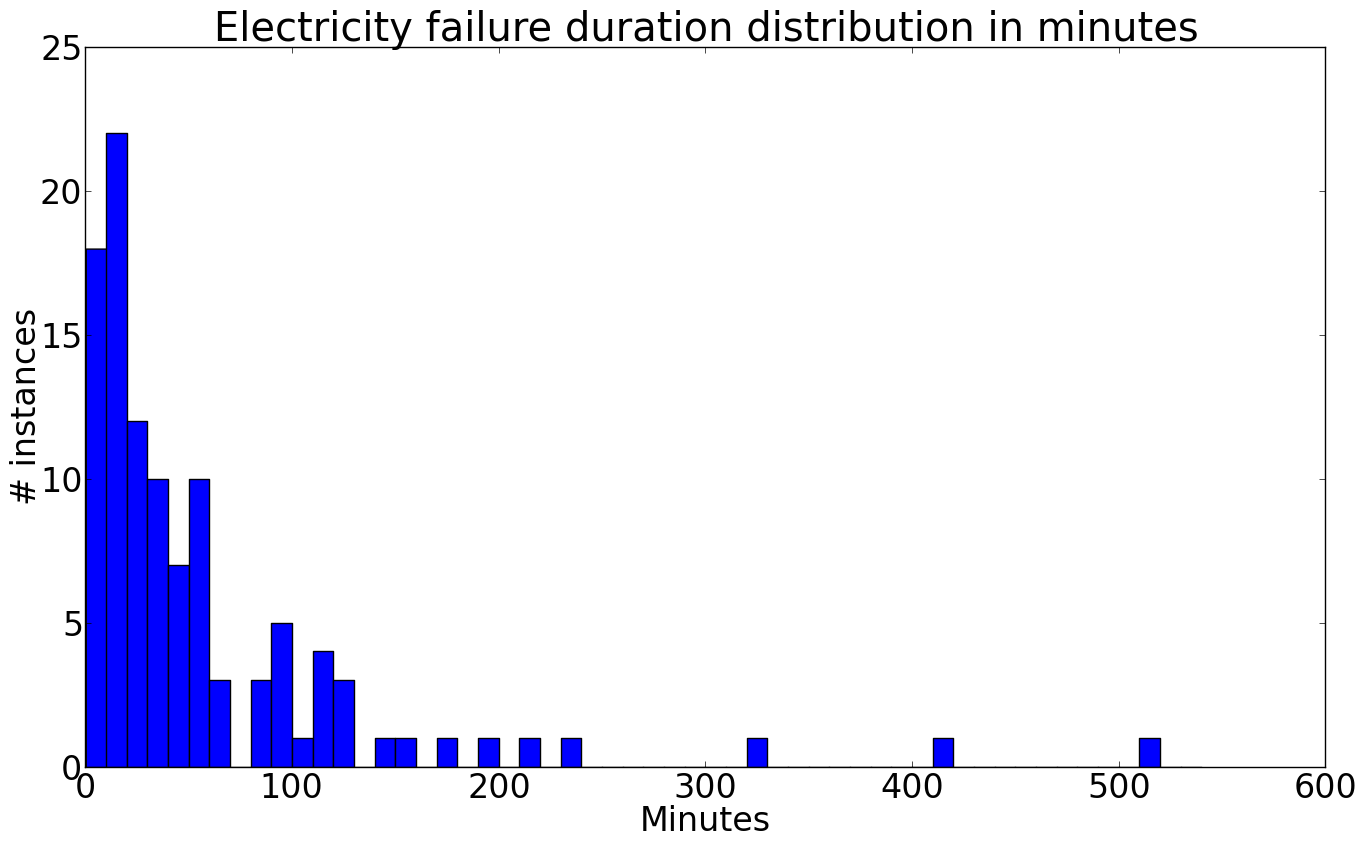
\includegraphics[scale=0.15]{./figures/failure_durations.png}}
       \hspace{1mm}
     \subfloat[\scriptsize Electricity failure by hour of day]{
             \label{fig:failure_hour}
             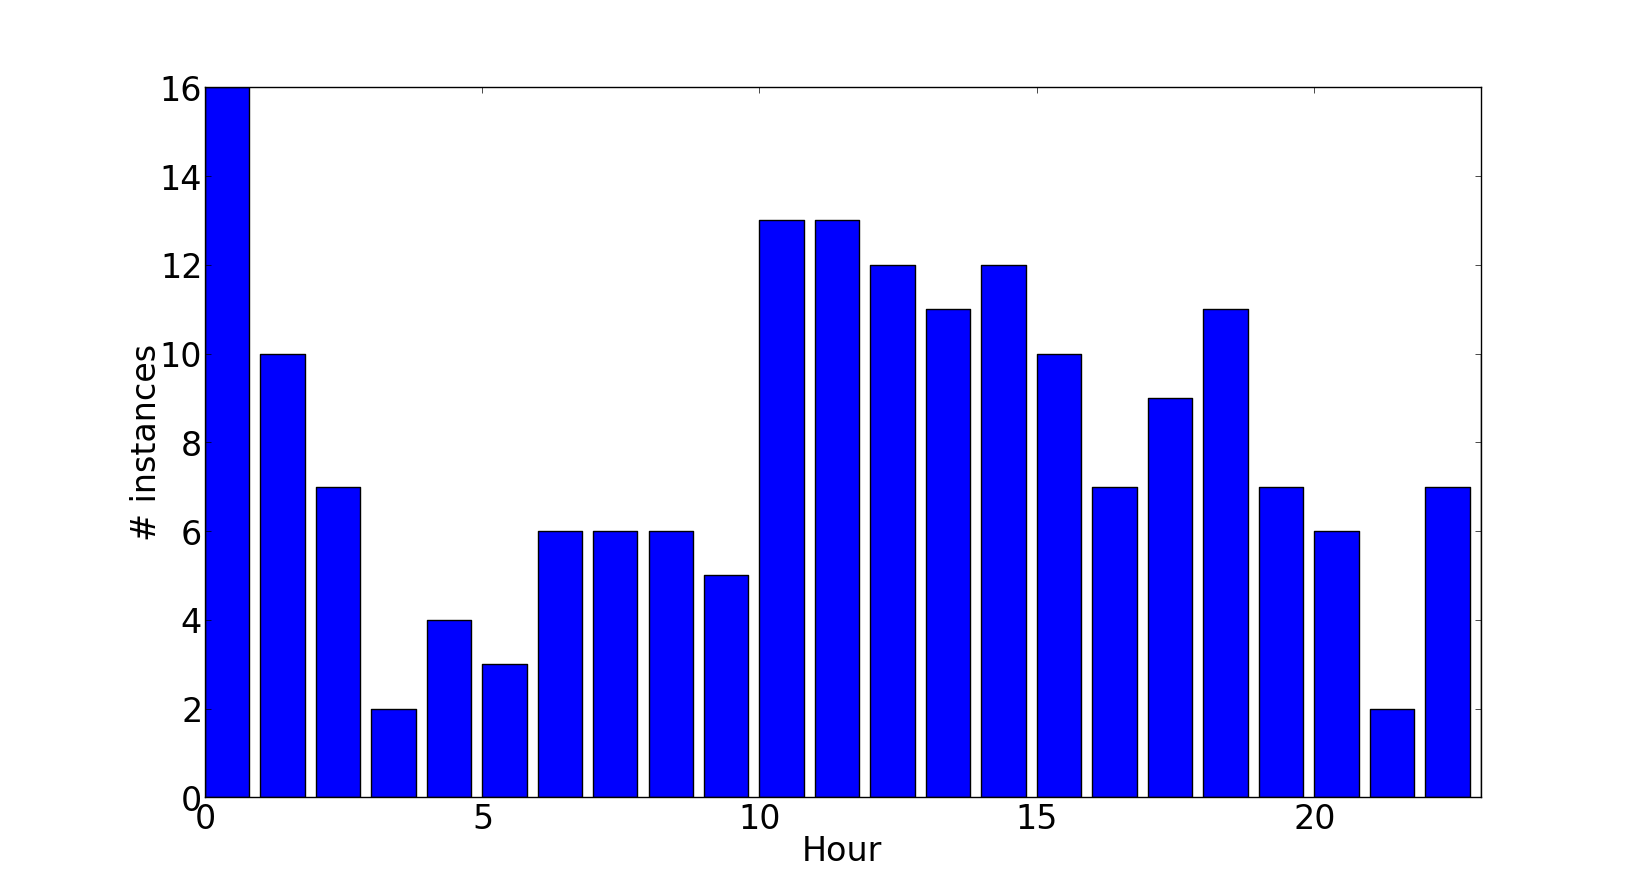
\includegraphics[scale=0.15]{./figures/failure_by_hour}}
              \vspace{-4mm}
             \newline
            
          \subfloat[\scriptsize Voltage fluctuations in a typical day]{
                  \label{fig:voltage}
                  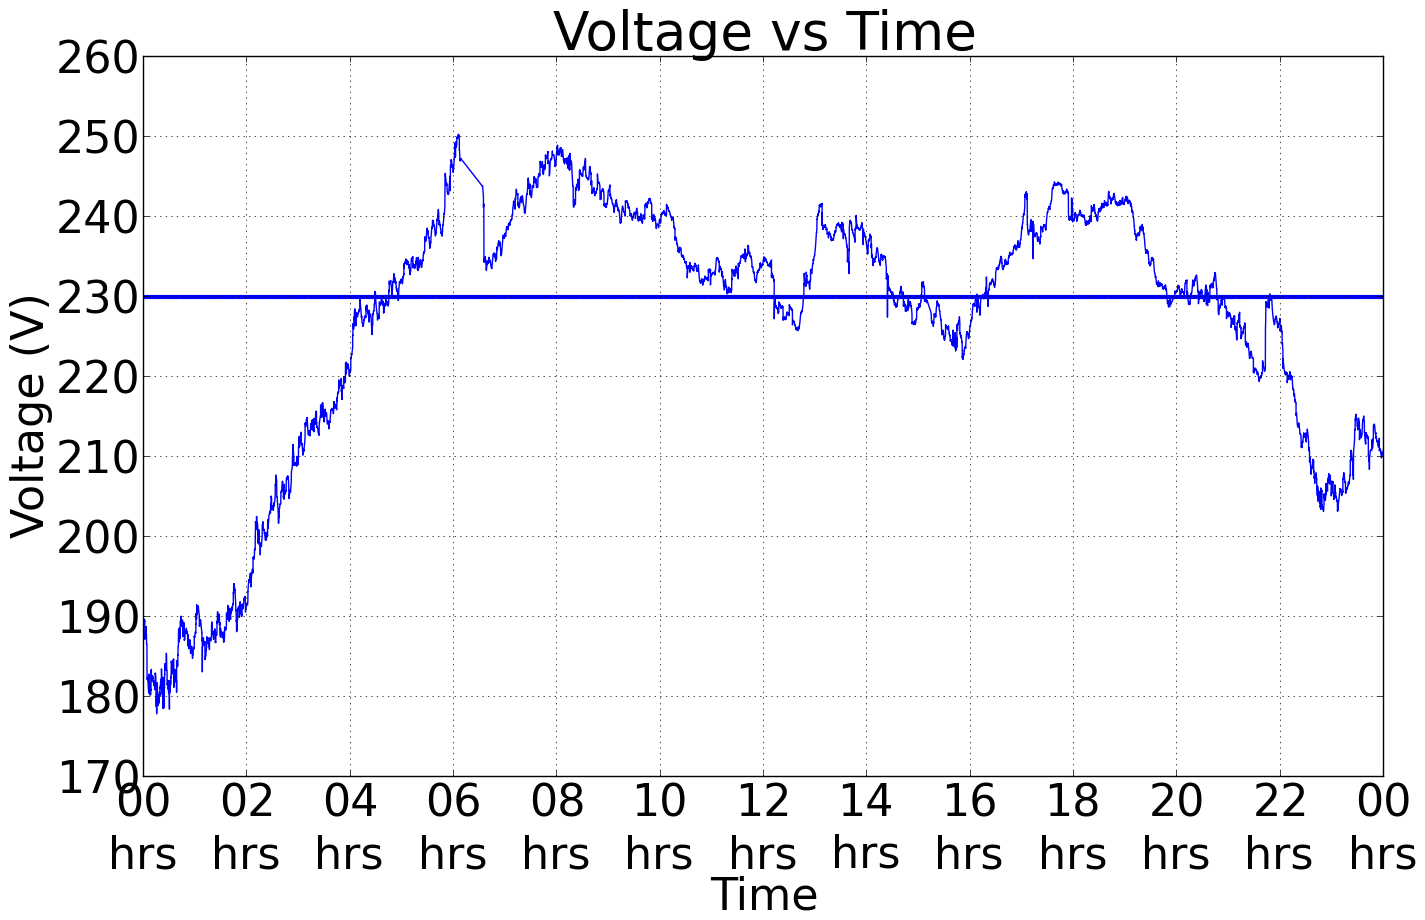
\includegraphics[scale=0.15]{./figures/voltage.png}}
          \subfloat[\scriptsize Frequency fluctuations in a typical day]{
                            \label{fig:frequency}
                            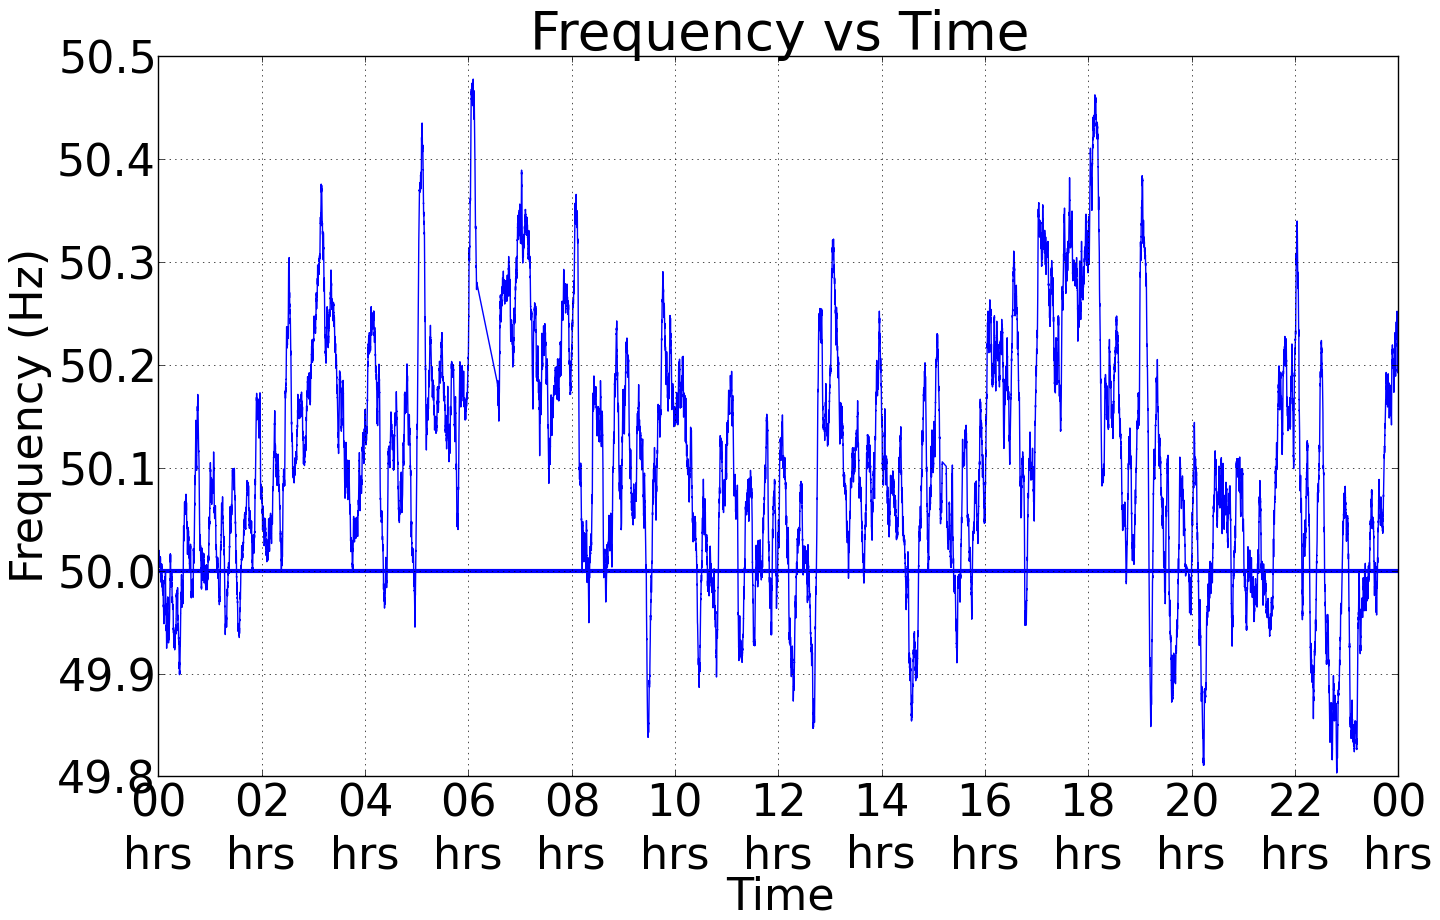
\includegraphics[scale=0.15]{./figures/frequency.png}}
          \subfloat[\scriptsize \% internet packet drop]{
                            \label{fig:network}
                            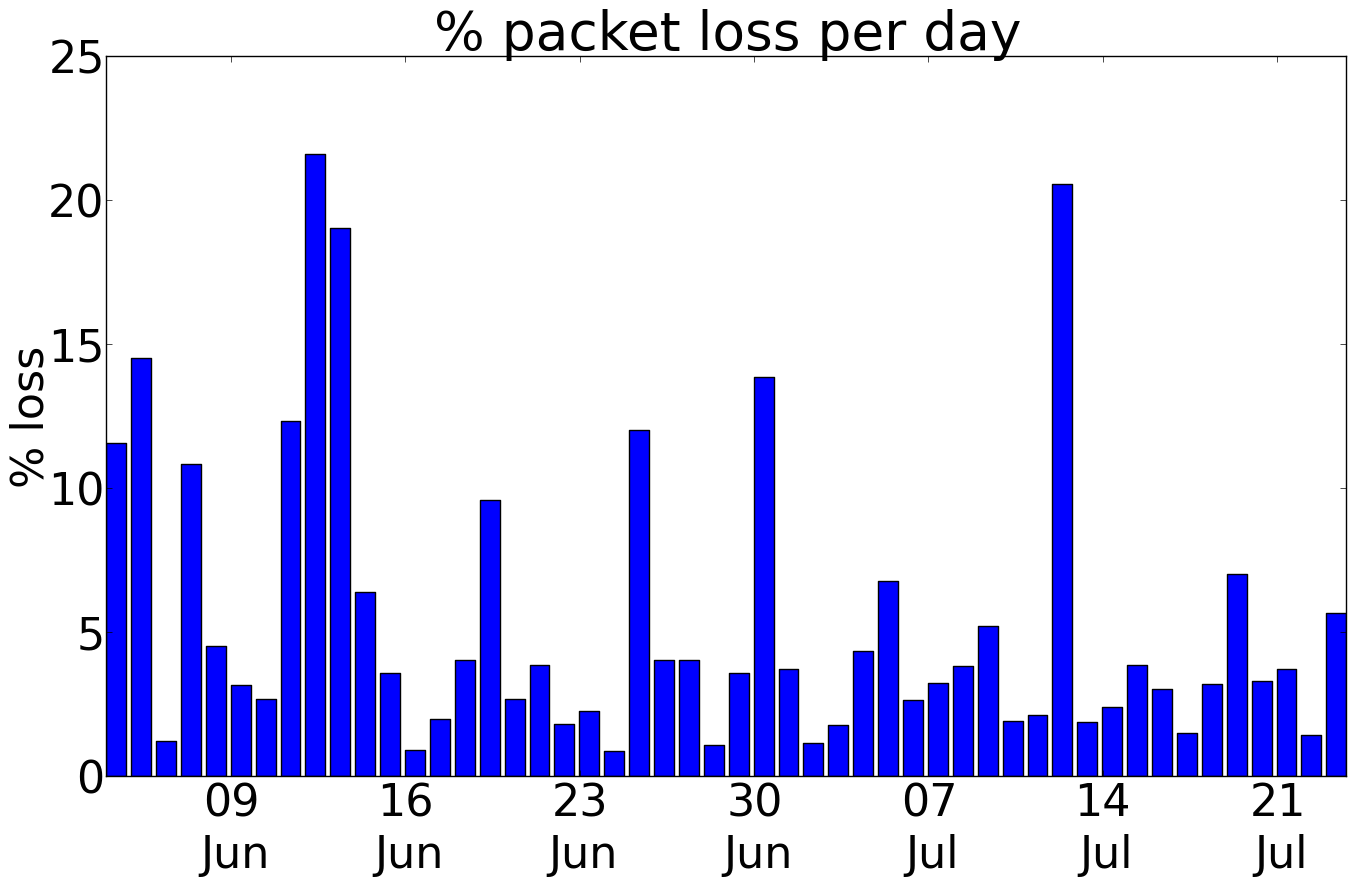
\includegraphics[scale=0.15]{./figures/network.png}}
   
    \caption{Unreliable internet and grid}

    \label{fig:unreliable}

\end{figure*}

\begin{figure}     
    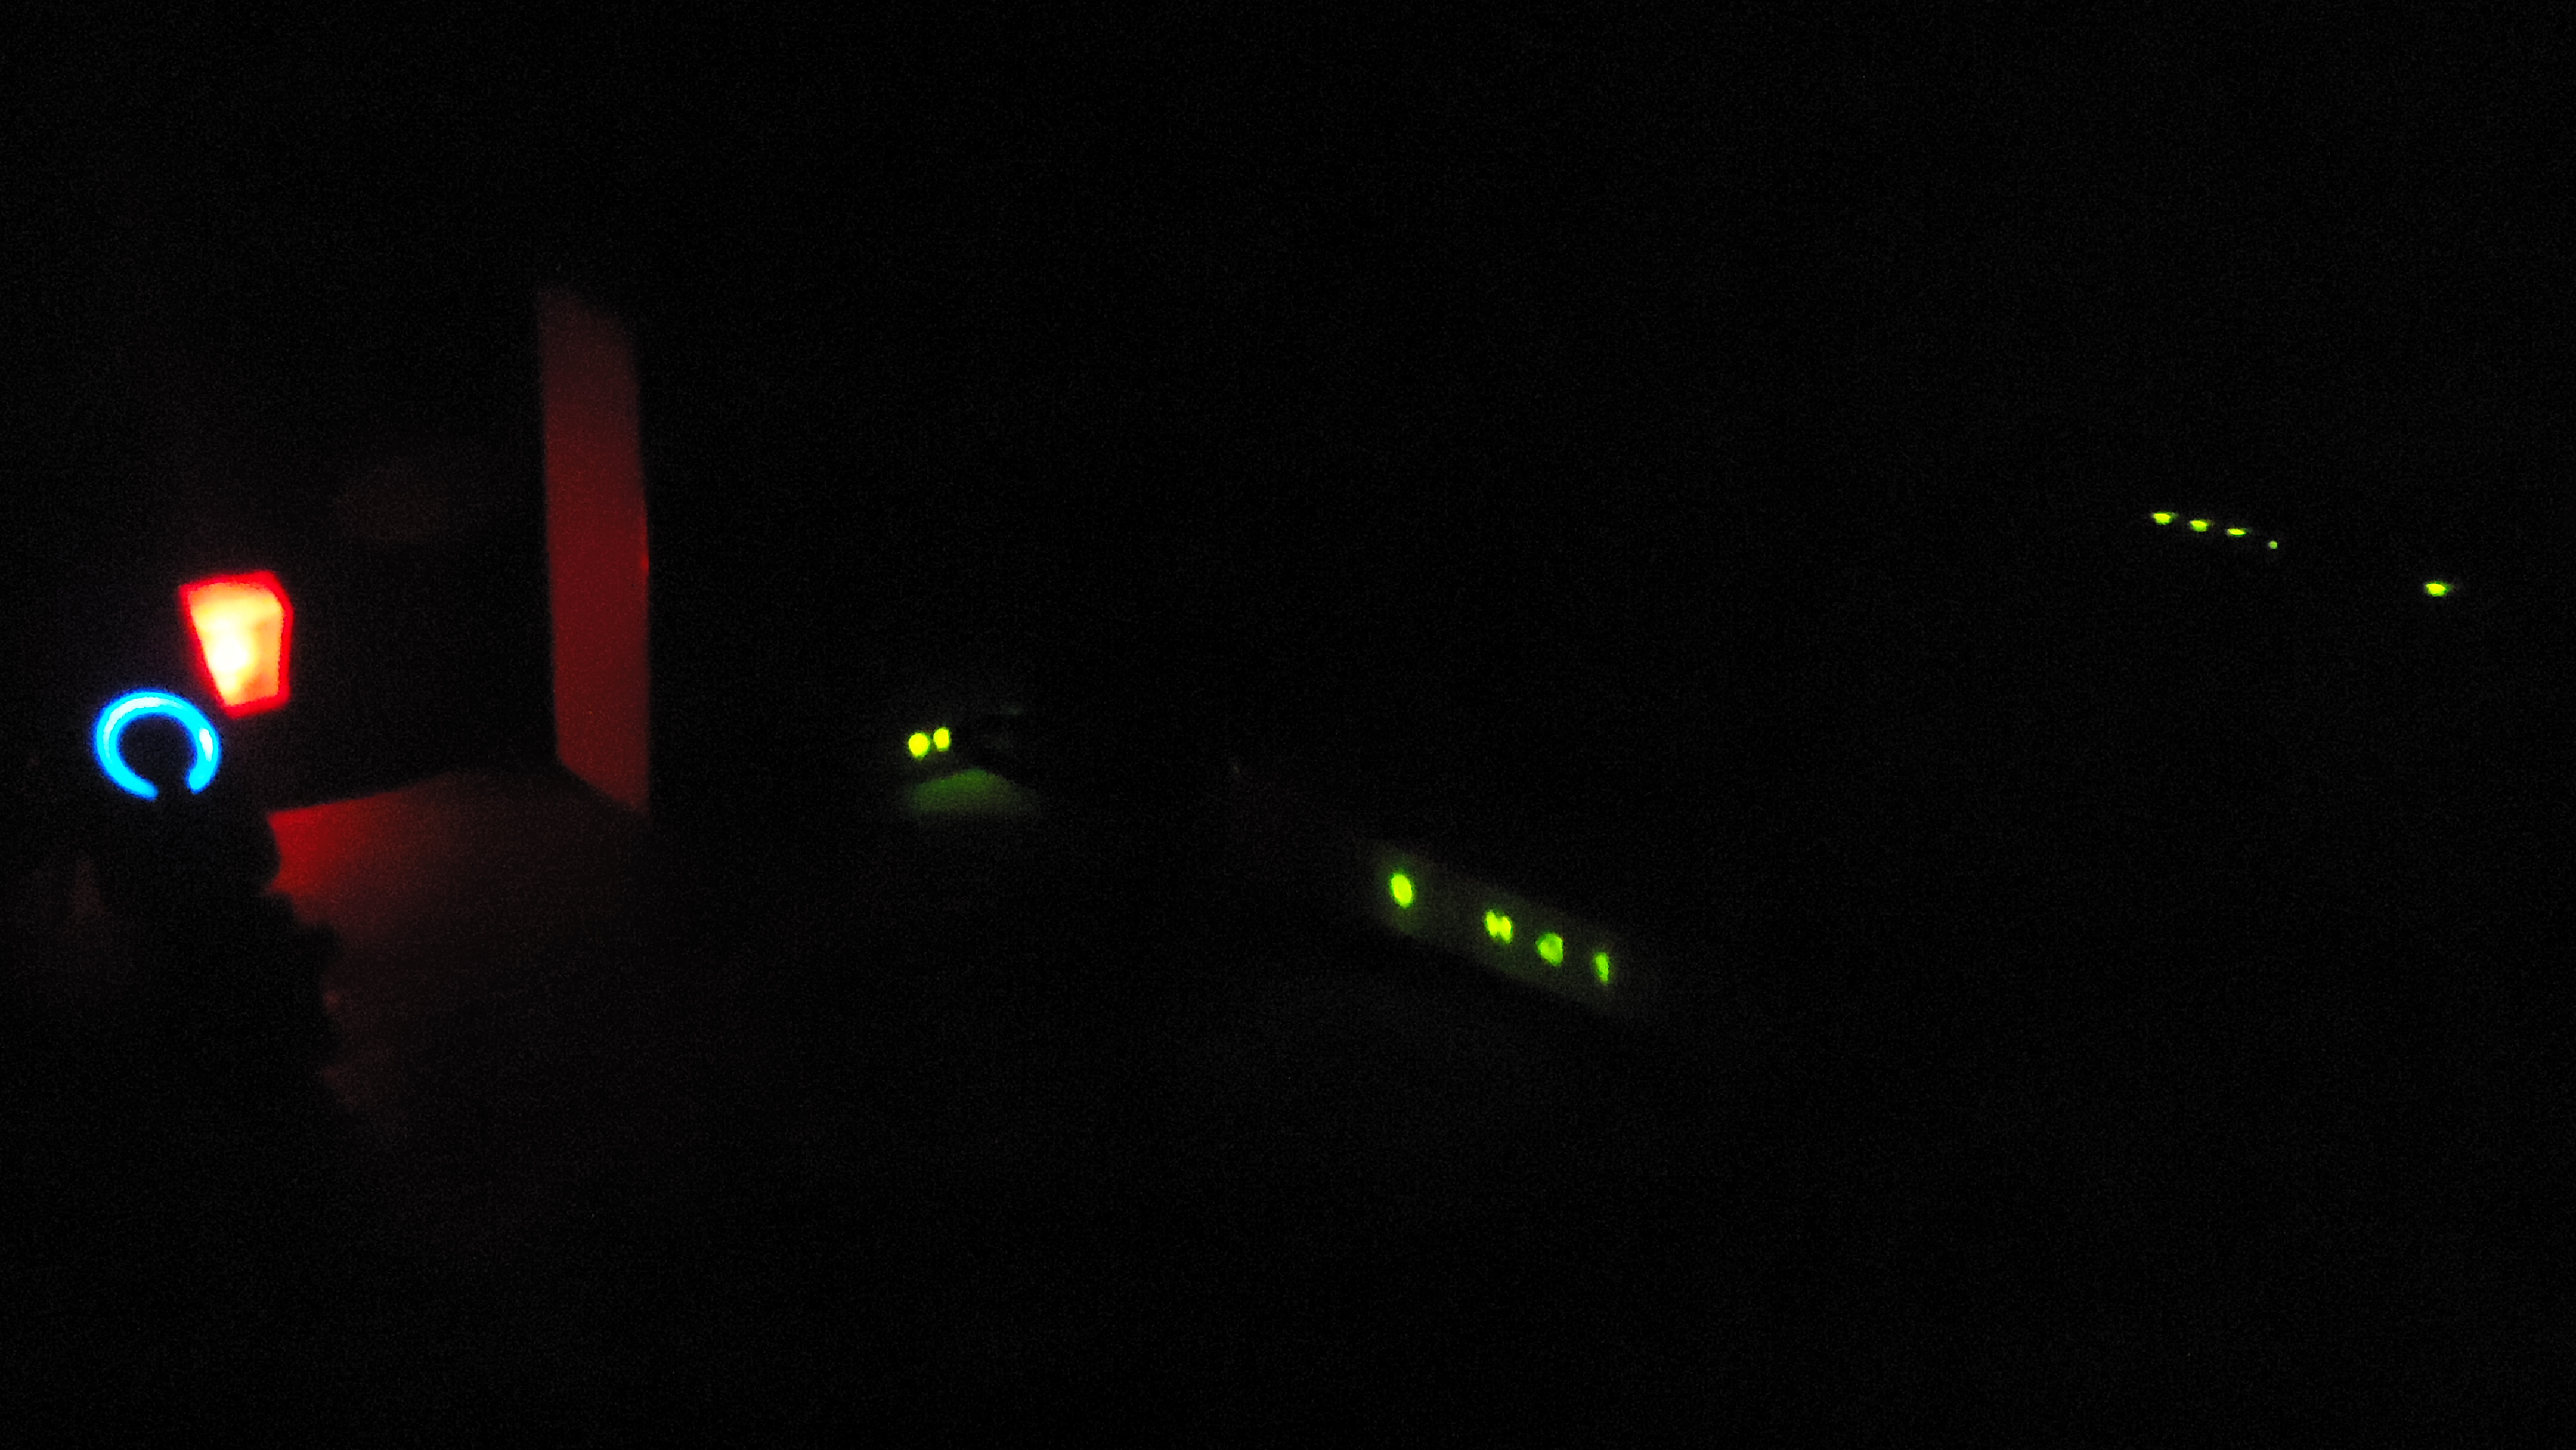
\includegraphics[scale=0.02]{./figures/led.JPG}    
    \caption{LED glowing in the night}   
    \label{fig:led}
   
\end{figure}

\section{Case Studies}
In this section we present some case studies from the data collected in this deployment.
\subsection{Correlating Events and Activity Detection}
In this section we show how multi-modal data can be used for activity recognition. Following plots show the same.


\subsection{Water-Energy Nexus}
\subsubsection{Water Filter}
In this section we find out the effective cost of 1 litre of water. RO is known to waste a lot of water. From the water meter we observe the amount of water consumed to fill 1 litre of water. We also see the corresponding power draw of the RO. Thus, we can see that water has energy embedded in it.

\subsubsection{Electric Motor}
Another unique aspect of our setting is the use of electric motor to pump water. Figure showing 1 litre events before motor was turned on and figure showing 1 litre events after motor is turned on.
Figure showing power consumption incurred by the use of motor.

\subsection{Energy conscious habits}
Figure showing how i turn the AC at 16 degrees and turn it off before going to sleep.

Running the ref. in least cool cooling mode and the impact it has.

\subsection{NILM}
Will be tough to do in timeframe.

To highlight any thing or add new stuff write like this in red

\redcolor{This is my comment. I would also do ... and put this image and put this table and so on and so forth}

\section{Conclusions and Future Work}


\balance
\bibliographystyle{abbrv}
\bibliography{references}  % sigproc.bib is the name of the Bibliography in this case
\end{document}
